% Options for packages loaded elsewhere
\PassOptionsToPackage{unicode}{hyperref}
\PassOptionsToPackage{hyphens}{url}
%
\documentclass[
  man]{apa6}
\usepackage{amsmath,amssymb}
\usepackage{lmodern}
\usepackage{iftex}
\ifPDFTeX
  \usepackage[T1]{fontenc}
  \usepackage[utf8]{inputenc}
  \usepackage{textcomp} % provide euro and other symbols
\else % if luatex or xetex
  \usepackage{unicode-math}
  \defaultfontfeatures{Scale=MatchLowercase}
  \defaultfontfeatures[\rmfamily]{Ligatures=TeX,Scale=1}
\fi
% Use upquote if available, for straight quotes in verbatim environments
\IfFileExists{upquote.sty}{\usepackage{upquote}}{}
\IfFileExists{microtype.sty}{% use microtype if available
  \usepackage[]{microtype}
  \UseMicrotypeSet[protrusion]{basicmath} % disable protrusion for tt fonts
}{}
\makeatletter
\@ifundefined{KOMAClassName}{% if non-KOMA class
  \IfFileExists{parskip.sty}{%
    \usepackage{parskip}
  }{% else
    \setlength{\parindent}{0pt}
    \setlength{\parskip}{6pt plus 2pt minus 1pt}}
}{% if KOMA class
  \KOMAoptions{parskip=half}}
\makeatother
\usepackage{xcolor}
\usepackage{color}
\usepackage{fancyvrb}
\newcommand{\VerbBar}{|}
\newcommand{\VERB}{\Verb[commandchars=\\\{\}]}
\DefineVerbatimEnvironment{Highlighting}{Verbatim}{commandchars=\\\{\}}
% Add ',fontsize=\small' for more characters per line
\usepackage{framed}
\definecolor{shadecolor}{RGB}{248,248,248}
\newenvironment{Shaded}{\begin{snugshade}}{\end{snugshade}}
\newcommand{\AlertTok}[1]{\textcolor[rgb]{0.94,0.16,0.16}{#1}}
\newcommand{\AnnotationTok}[1]{\textcolor[rgb]{0.56,0.35,0.01}{\textbf{\textit{#1}}}}
\newcommand{\AttributeTok}[1]{\textcolor[rgb]{0.77,0.63,0.00}{#1}}
\newcommand{\BaseNTok}[1]{\textcolor[rgb]{0.00,0.00,0.81}{#1}}
\newcommand{\BuiltInTok}[1]{#1}
\newcommand{\CharTok}[1]{\textcolor[rgb]{0.31,0.60,0.02}{#1}}
\newcommand{\CommentTok}[1]{\textcolor[rgb]{0.56,0.35,0.01}{\textit{#1}}}
\newcommand{\CommentVarTok}[1]{\textcolor[rgb]{0.56,0.35,0.01}{\textbf{\textit{#1}}}}
\newcommand{\ConstantTok}[1]{\textcolor[rgb]{0.00,0.00,0.00}{#1}}
\newcommand{\ControlFlowTok}[1]{\textcolor[rgb]{0.13,0.29,0.53}{\textbf{#1}}}
\newcommand{\DataTypeTok}[1]{\textcolor[rgb]{0.13,0.29,0.53}{#1}}
\newcommand{\DecValTok}[1]{\textcolor[rgb]{0.00,0.00,0.81}{#1}}
\newcommand{\DocumentationTok}[1]{\textcolor[rgb]{0.56,0.35,0.01}{\textbf{\textit{#1}}}}
\newcommand{\ErrorTok}[1]{\textcolor[rgb]{0.64,0.00,0.00}{\textbf{#1}}}
\newcommand{\ExtensionTok}[1]{#1}
\newcommand{\FloatTok}[1]{\textcolor[rgb]{0.00,0.00,0.81}{#1}}
\newcommand{\FunctionTok}[1]{\textcolor[rgb]{0.00,0.00,0.00}{#1}}
\newcommand{\ImportTok}[1]{#1}
\newcommand{\InformationTok}[1]{\textcolor[rgb]{0.56,0.35,0.01}{\textbf{\textit{#1}}}}
\newcommand{\KeywordTok}[1]{\textcolor[rgb]{0.13,0.29,0.53}{\textbf{#1}}}
\newcommand{\NormalTok}[1]{#1}
\newcommand{\OperatorTok}[1]{\textcolor[rgb]{0.81,0.36,0.00}{\textbf{#1}}}
\newcommand{\OtherTok}[1]{\textcolor[rgb]{0.56,0.35,0.01}{#1}}
\newcommand{\PreprocessorTok}[1]{\textcolor[rgb]{0.56,0.35,0.01}{\textit{#1}}}
\newcommand{\RegionMarkerTok}[1]{#1}
\newcommand{\SpecialCharTok}[1]{\textcolor[rgb]{0.00,0.00,0.00}{#1}}
\newcommand{\SpecialStringTok}[1]{\textcolor[rgb]{0.31,0.60,0.02}{#1}}
\newcommand{\StringTok}[1]{\textcolor[rgb]{0.31,0.60,0.02}{#1}}
\newcommand{\VariableTok}[1]{\textcolor[rgb]{0.00,0.00,0.00}{#1}}
\newcommand{\VerbatimStringTok}[1]{\textcolor[rgb]{0.31,0.60,0.02}{#1}}
\newcommand{\WarningTok}[1]{\textcolor[rgb]{0.56,0.35,0.01}{\textbf{\textit{#1}}}}
\usepackage{longtable,booktabs,array}
\usepackage{calc} % for calculating minipage widths
% Correct order of tables after \paragraph or \subparagraph
\usepackage{etoolbox}
\makeatletter
\patchcmd\longtable{\par}{\if@noskipsec\mbox{}\fi\par}{}{}
\makeatother
% Allow footnotes in longtable head/foot
\IfFileExists{footnotehyper.sty}{\usepackage{footnotehyper}}{\usepackage{footnote}}
\makesavenoteenv{longtable}
\usepackage{graphicx}
\makeatletter
\def\maxwidth{\ifdim\Gin@nat@width>\linewidth\linewidth\else\Gin@nat@width\fi}
\def\maxheight{\ifdim\Gin@nat@height>\textheight\textheight\else\Gin@nat@height\fi}
\makeatother
% Scale images if necessary, so that they will not overflow the page
% margins by default, and it is still possible to overwrite the defaults
% using explicit options in \includegraphics[width, height, ...]{}
\setkeys{Gin}{width=\maxwidth,height=\maxheight,keepaspectratio}
% Set default figure placement to htbp
\makeatletter
\def\fps@figure{htbp}
\makeatother
\setlength{\emergencystretch}{3em} % prevent overfull lines
\providecommand{\tightlist}{%
  \setlength{\itemsep}{0pt}\setlength{\parskip}{0pt}}
\setcounter{secnumdepth}{-\maxdimen} % remove section numbering
% Make \paragraph and \subparagraph free-standing
\ifx\paragraph\undefined\else
  \let\oldparagraph\paragraph
  \renewcommand{\paragraph}[1]{\oldparagraph{#1}\mbox{}}
\fi
\ifx\subparagraph\undefined\else
  \let\oldsubparagraph\subparagraph
  \renewcommand{\subparagraph}[1]{\oldsubparagraph{#1}\mbox{}}
\fi
\newlength{\cslhangindent}
\setlength{\cslhangindent}{1.5em}
\newlength{\csllabelwidth}
\setlength{\csllabelwidth}{3em}
\newlength{\cslentryspacingunit} % times entry-spacing
\setlength{\cslentryspacingunit}{\parskip}
\newenvironment{CSLReferences}[2] % #1 hanging-ident, #2 entry spacing
 {% don't indent paragraphs
  \setlength{\parindent}{0pt}
  % turn on hanging indent if param 1 is 1
  \ifodd #1
  \let\oldpar\par
  \def\par{\hangindent=\cslhangindent\oldpar}
  \fi
  % set entry spacing
  \setlength{\parskip}{#2\cslentryspacingunit}
 }%
 {}
\usepackage{calc}
\newcommand{\CSLBlock}[1]{#1\hfill\break}
\newcommand{\CSLLeftMargin}[1]{\parbox[t]{\csllabelwidth}{#1}}
\newcommand{\CSLRightInline}[1]{\parbox[t]{\linewidth - \csllabelwidth}{#1}\break}
\newcommand{\CSLIndent}[1]{\hspace{\cslhangindent}#1}
\ifLuaTeX
\usepackage[bidi=basic]{babel}
\else
\usepackage[bidi=default]{babel}
\fi
\babelprovide[main,import]{english}
% get rid of language-specific shorthands (see #6817):
\let\LanguageShortHands\languageshorthands
\def\languageshorthands#1{}
% Manuscript styling
\usepackage{upgreek}
\captionsetup{font=singlespacing,justification=justified}

% Table formatting
\usepackage{longtable}
\usepackage{lscape}
% \usepackage[counterclockwise]{rotating}   % Landscape page setup for large tables
\usepackage{multirow}		% Table styling
\usepackage{tabularx}		% Control Column width
\usepackage[flushleft]{threeparttable}	% Allows for three part tables with a specified notes section
\usepackage{threeparttablex}            % Lets threeparttable work with longtable

% Create new environments so endfloat can handle them
% \newenvironment{ltable}
%   {\begin{landscape}\centering\begin{threeparttable}}
%   {\end{threeparttable}\end{landscape}}
\newenvironment{lltable}{\begin{landscape}\centering\begin{ThreePartTable}}{\end{ThreePartTable}\end{landscape}}

% Enables adjusting longtable caption width to table width
% Solution found at http://golatex.de/longtable-mit-caption-so-breit-wie-die-tabelle-t15767.html
\makeatletter
\newcommand\LastLTentrywidth{1em}
\newlength\longtablewidth
\setlength{\longtablewidth}{1in}
\newcommand{\getlongtablewidth}{\begingroup \ifcsname LT@\roman{LT@tables}\endcsname \global\longtablewidth=0pt \renewcommand{\LT@entry}[2]{\global\advance\longtablewidth by ##2\relax\gdef\LastLTentrywidth{##2}}\@nameuse{LT@\roman{LT@tables}} \fi \endgroup}

% \setlength{\parindent}{0.5in}
% \setlength{\parskip}{0pt plus 0pt minus 0pt}

% Overwrite redefinition of paragraph and subparagraph by the default LaTeX template
% See https://github.com/crsh/papaja/issues/292
\makeatletter
\renewcommand{\paragraph}{\@startsection{paragraph}{4}{\parindent}%
  {0\baselineskip \@plus 0.2ex \@minus 0.2ex}%
  {-1em}%
  {\normalfont\normalsize\bfseries\itshape\typesectitle}}

\renewcommand{\subparagraph}[1]{\@startsection{subparagraph}{5}{1em}%
  {0\baselineskip \@plus 0.2ex \@minus 0.2ex}%
  {-\z@\relax}%
  {\normalfont\normalsize\itshape\hspace{\parindent}{#1}\textit{\addperi}}{\relax}}
\makeatother

% \usepackage{etoolbox}
\makeatletter
\patchcmd{\HyOrg@maketitle}
  {\section{\normalfont\normalsize\abstractname}}
  {\section*{\normalfont\normalsize\abstractname}}
  {}{\typeout{Failed to patch abstract.}}
\patchcmd{\HyOrg@maketitle}
  {\section{\protect\normalfont{\@title}}}
  {\section*{\protect\normalfont{\@title}}}
  {}{\typeout{Failed to patch title.}}
\makeatother

\usepackage{xpatch}
\makeatletter
\xapptocmd\appendix
  {\xapptocmd\section
    {\addcontentsline{toc}{section}{\appendixname\ifoneappendix\else~\theappendix\fi\\: #1}}
    {}{\InnerPatchFailed}%
  }
{}{\PatchFailed}
\keywords{long range correlation, fractal, multiscale, dynamical systems\newline\indent Word count: 6,888}
\DeclareDelayedFloatFlavor{ThreePartTable}{table}
\DeclareDelayedFloatFlavor{lltable}{table}
\DeclareDelayedFloatFlavor*{longtable}{table}
\makeatletter
\renewcommand{\efloat@iwrite}[1]{\immediate\expandafter\protected@write\csname efloat@post#1\endcsname{}}
\makeatother
\usepackage{lineno}

\linenumbers
\usepackage{csquotes}
\ifLuaTeX
  \usepackage{selnolig}  % disable illegal ligatures
\fi
\IfFileExists{bookmark.sty}{\usepackage{bookmark}}{\usepackage{hyperref}}
\IfFileExists{xurl.sty}{\usepackage{xurl}}{} % add URL line breaks if available
\urlstyle{same} % disable monospaced font for URLs
\hypersetup{
  pdftitle={fractalRegression: An R package for multiscale regression and fractal analyses},
  pdfauthor={Aaron D. Likens1 \& Travis J. Wiltshire2},
  pdflang={en-EN},
  pdfkeywords={long range correlation, fractal, multiscale, dynamical systems},
  hidelinks,
  pdfcreator={LaTeX via pandoc}}

\title{fractalRegression: An R package for multiscale regression and fractal analyses}
\author{Aaron D. Likens\textsuperscript{1} \& Travis J. Wiltshire\textsuperscript{2}}
\date{}


\shorttitle{FRACTAL REGRESSION}

\authornote{

The authors made the following contributions. Aaron D. Likens: Conceptualization, Software, Writing - Original Draft Preparation, Writing - Review \& Editing; Travis J. Wiltshire: Writing - Original Draft Preparation, Writing - Review \& Editing, Software.

Correspondence concerning this article should be addressed to Aaron D. Likens, Division of Biomechanics and Research Development, Department of Biomechanics, and Center for Research in Human Movement Variability, University of Nebraska at Omaha,6160 University Dr S,Omaha, 68182, NE, USA.. E-mail: \href{mailto:alikens@unomaha.edu}{\nolinkurl{alikens@unomaha.edu}}

}

\affiliation{\vspace{0.5cm}\textsuperscript{1} Department of Biomechanics, University of Nebraska at Omaha\\\textsuperscript{2} Department of Cognitive Science \& Artificial Intelligence, Tilburg University}

\abstract{%
Time series data from scientific fields as diverse as astrophysics, economics, human movement science, and neuroscience all exhibit fractal properties. That is, these time series often exhibit self-similarity and long-range correlations. This \texttt{fractalRegression} package implements a number of univariate and bivariate time series tools appropriate for analyzing noisy data exhibiting these properties. These methods, especially the bivariate tools (Kristoufek, 2015a; Likens, Amazeen, West, \& Gibbons, 2019a) have yet to be implemented in an open source and complete package for the R Statistical Software environment. As both practitioners and developers of these methods, we expect these tools will be of interest to a wide audience of scientists who use R, especially those from fields such as the human movement, cognitive, and other behavioral sciences. The algorithms have been developed in C++ using the popular Rcpp (Eddelbuettel \& Francois, 2011) and RcppArmadillo (Eddelbuettel \& Sanderson, 2014) packages. The result is a collection of efficient functions that perform well even on long time series (e.g., \(\geq\) 10,000 data points). In this work, we introduce the package, each of the functions, and give examples of their use as well as issues to consider to correctly use these methods.
}



\begin{document}
\maketitle

\hypertarget{introduction}{%
\section{Introduction}\label{introduction}}

Over time, many signals from living and complex systems exhibit
systematic regularities and dependencies across spatial and temporal
scales (Kello et al., 2010). These regularities often follow
a power-law (i.e., self-similarity across scales) that are estimated
using fractal analyses. Fractal analysis, in its many forms, has become
an important framework in virtually every area of science, often serving
as an indicator of system health
(Goldberger et al., 2002), adaptability
(Bak, Tang, \& Wiesenfeld, 1987), control
(Likens, Fine, Amazeen, \& Amazeen, 2015), cognitive function
(Euler, Wiltshire, Niermeyer, \& Butner, 2016), and multi-scale interactions
(Kelty-Stephen, 2017).

In particular, various methods related to Detrended Fluctuation Analysis
(DFA) (Peng et al., 1994) have rose to prominence due to
their relative ease of understanding and broad applicability to
stationary and non-stationary time series, alike. More specifically, in
areas of the social and cognitive sciences, DFA, or variants of DFA,
have been used to study, for example, reaction times
(Van Orden, Holden, \& Turvey, 2003), eye gaze
(Stephen, Boncoddo, Magnuson, \& Dixon, 2009), gait
(Delignières \& Torre, 2009; Hausdorff et al., 1996), limb movements
(Delignières, Torre, \& Lemoine, 2008), heart rate
(Goldberger et al., 2002), and neurophysiological
oscillations (Euler et al., 2016; Hardstone et al., 2012; Schaworonkow \& Voytek, 2021). And, beyond an individual level,
the methods have been used to study human-machine system interaction
(Likens et al., 2015), tool use
(Favela, 2020; Kelty-Stephen, Stirling, \& Lipsitz, 2016), and interpersonal coordination
in a variety of modalities
(Davis, Brooks, \& Dixon, 2016; Delignières, Almurad, Roume, \& Marmelat, 2016).

Thus, there is a broad scientific appeal for these fractal-based
analyses. While, the basic DFA algorithm has been implemented in
numerous packages and software programs, more advanced methods such as
Multifractal Detrended Fluctuation Analysis (MFDFA)
(Kantelhardt et al., 2002), Detrended Cross
Correlation Analysis (DCCA)
(Podobnik \& Stanley, 2008; Zebende, 2011), and, in particular,
fractal regression techniques such as Multiscale Regression Analysis
(MRA) (Kristoufek, 2015a; Likens et al., 2019a) have not yet been
implemented in a comprehensive software package. A key aspect of this
effort is to draw more attention and make more available these \emph{fractal
regression} techniques. In particular, we find these methods widely
promising because they allow for uncovering ``the time scales most
relevant to relationships between a system's components'' (p.~2) within a
predictive framework (Likens et al., 2019a).

Thus, there is a clear need for a package that incorporates this
functionality in order to advance theoretical research focused on
understanding the time varying properties of natural phenomena and
applied research that uses those insights in important and diverse areas
such as healthcare (Cavanaugh, Kelty-Stephen, \& Stergiou, 2017) and education (Snow, Likens, Allen, \& McNamara, 2016). In this
work, we provide an overview of our \texttt{fractalRegression} package, provide
simulated and empirical examples of its functions, and provide practical
advice on the successful application of these methods.

\hypertarget{package-overview}{%
\section{Package Overview}\label{package-overview}}

Our \texttt{fractalRegression} package for R
(Team, 2018) is built on a C++
architecture and includes a variety of uni- and bivariate fractal
methods as well as functions for simulating data with known fractional
properties (e.g., scaling, dependence, etc.), and surrogate testing.
Some foundational efforts in fractal analyses, which partially overlap
with the functionality of this package, have been implemented elsewhere.
For example, a number of univariate fractal and multifractal analyses
have been implemented in the `fracLab' library for MATLAB (Legrand \& Véhel, 2003)
and other toolboxes that are mainly targeted at multifractal analysis
(Ihlen, 2012; Ihlen \& Vereijken, 2010). In terms of
open access packages, there are other packages that implement some, but
not all of the same functions such as the \texttt{fathon} package
(Bianchi, 2020) that has been implemented in Python as well as the R
packages: \texttt{fractal} {[}defunct{]}, \texttt{nonlinearTseries}
(Garcia, 2020), and \texttt{MFDFA}
(Laib, Golay, Telesca, \& Kanevski, 2018). However, none of the above packages
incorporate univariate monofractal and multifractal DFA with bivariate
DCCA and MRA and some are only written in base R code, which can be less
efficient for long time series. Our \texttt{fractalRegression} package is
unique in this combination of analyses and efficiency (particularly for
long time series). For instance, we are not aware of any other packages
that feature MRA. In addition, we expect that featuring simulation
methods as well as surrogate testing strongly bolsters the accessibility
of these methods for the social and cognitive science community in
particular, but also science, more generally. An overview of the core
functions included in the package, the general objective of that
function, and the output are shown below in Table 1. Note that there are
some additional helper and plotting functions included as well. The
additional details are included in the sections corresponding to those
methods, in the package documentation, and in the original sources for
the methods.

\textbf{Table 1.}

\emph{Overview of core package functions, objectives, and output}

\begin{longtable}[]{@{}
  >{\raggedright\arraybackslash}p{(\columnwidth - 4\tabcolsep) * \real{0.2603}}
  >{\raggedright\arraybackslash}p{(\columnwidth - 4\tabcolsep) * \real{0.2603}}
  >{\raggedright\arraybackslash}p{(\columnwidth - 4\tabcolsep) * \real{0.4795}}@{}}
\caption{\textbf{Table 1.} \emph{Overview of core package functions, objectives, and
output}}\tabularnewline
\toprule()
\begin{minipage}[b]{\linewidth}\raggedright
Function
\end{minipage} & \begin{minipage}[b]{\linewidth}\raggedright
Objective
\end{minipage} & \begin{minipage}[b]{\linewidth}\raggedright
Output
\end{minipage} \\
\midrule()
\endfirsthead
\toprule()
\begin{minipage}[b]{\linewidth}\raggedright
Function
\end{minipage} & \begin{minipage}[b]{\linewidth}\raggedright
Objective
\end{minipage} & \begin{minipage}[b]{\linewidth}\raggedright
Output
\end{minipage} \\
\midrule()
\endhead
\texttt{dfa()} & Estimate long-range correlation in a time series & Object containing the overall \(\alpha\) estimate and, if desired the \texttt{logScales} and \texttt{logRMS} \\
\texttt{mfdfa()} & Estimate the magnitude and range of long-range correlations in a time series & Object containing the \(\log\) scales used for the analysis, the \(\log\) fluctuation function for each scale and \(q\), the various q-order exponents, \(Hq\), \(Tau\), \(h\), and \(Dh\). The base of \(log\) depends on scale construction and user input \\
\texttt{dcca()} & Estimates of scale-specific correlation between two time-series & Object containing the scales used for the analysis and the \(\rho\) '\texttt{rho\textquotesingle{}} values for each scale \\
\texttt{mra()} & Estimates the scale specific regression coefficients for a predictor time series on and outcome time series & Object containing the scales and scale specific \(\beta\) estimates, \(R^2\), and \(t\) statistics \\
\texttt{fgn\_sim()} & Simulate univariate fractional Gaussian noise & Returns a vector of length \texttt{N} according to the specified \texttt{H} Hurst exponent \\
\texttt{mBm\_mGn()} & Simulate univariate multi-fractional Brownian motion and Gaussian noise & Returns two vectors of length \texttt{N} according to the specified \(H_t\) series \\
\texttt{mc\_ARFIMA()} & Simulate various types of bivariate correlated noise processes. & Returns two vectors of length \texttt{N} according to the specified noise \texttt{process} and parameters \\
\texttt{iaaft()} & Generate surrogate series using the iterative amplitude adjusted Fourier transform & Returns a vector of same length as input time series \\
\bottomrule()
\end{longtable}

\hypertarget{methodological-details-and-examples}{%
\section{Methodological Details and Examples}\label{methodological-details-and-examples}}

In order to demonstrate the methods within the \texttt{fractalRegression}
package, we group this into univariate (DFA, MFDFA) and bivariate
methods (DCCA, MRA). For each method, we 1) highlight the key
question(s) that can be answered with that method, 2) briefly describe
the algorithm with references to additional details (see also Appendix 1
for fundamental equations), 3) describe some key considerations for
appropriately applying the algorithm, and demonstrate the use of the
functions on a 4) simulated and 5) empirical example. Note that all
code, data, and text are part of a reproducible manuscript that are
accessible at the following link:
\url{https://github.com/travisjwiltshire/fractal_regression_manuscript}.

\hypertarget{univariate-methods}{%
\subsection{Univariate Methods}\label{univariate-methods}}

\hypertarget{detrended-fluctuation-analysis}{%
\subsubsection{Detrended Fluctuation Analysis}\label{detrended-fluctuation-analysis}}

A key question that can be answered by Detrended Fluctuation Analysis
(DFA) (Peng et al., 1994) is: \emph{what is the magnitude and
direction of long range correlation in a single time series?} While DFA
has been described extensively
(Kantelhardt, Koscielny-Bunde, Rego, Havlin, \& Bunde, 2001) and visualized nicely
elsewhere (Kelty-Stephen et al., 2016), we
provide a brief summary here. DFA entails splitting a time series into
several small bins (e.g., 16). In each bin, a least squares regression
is fit and subtracted within each window. Residuals are squared and
averaged within each window. Then, the square root is taken of the
average squared residual across all windows of a given size. This
process repeats for larger window sizes, growing by, say a power of 2,
up to \(N/4\), where \(N\) is the length of the series. In a final step, the
logarithm of those scaled root mean squared residuals (i.e.,
fluctuations) is regressed on the logarithm of window sizes. The slope
of this line is termed \(\alpha\) and it provides a measure of the long
range correlation. \(\alpha\) is commonly used an as estimator of the
Hurst exponent (\(H\)), where \(\alpha<1\) = \(H\), and for \(\alpha>1\),
\(H = 1 - \alpha\). Conventional interpretation of \(\alpha\) is:
\(\alpha < 0.5\) is anti-correlated, \(\alpha ~= 0.5\) is uncorrelated,
white noise, \(\alpha > 0.5\) is temporally correlated, \(\alpha ~= 1\) is
long-range correlated, 1/f-noise, pink noise, \(\alpha > 1\) is
non-stationary where the special case \(\alpha ~= 1.5\) is fractional
Brownian noise. More generally, \(1<\alpha<2\) are referred to as
fractional Brownian motion.

\hypertarget{dfa-examples}{%
\paragraph{DFA Examples}\label{dfa-examples}}

To demonstrate the use of \texttt{dfa()} we simulate three time series using
the \texttt{fgn\_sim()} function. This is a simple function based on the former
\texttt{fARMA} R package {[}defunct{]}. It requires the number of observations \texttt{n},
and the Hurst exponent \texttt{H}. In particular, we simulate white noise, pink
noise, and anti-correlated fractional Gaussian noise using the code
below.

\begin{Shaded}
\begin{Highlighting}[]
\NormalTok{white.noise }\OtherTok{\textless{}{-}} \FunctionTok{fgn\_sim}\NormalTok{(}\AttributeTok{n =} \DecValTok{5000}\NormalTok{, }\AttributeTok{H =} \FloatTok{0.5}\NormalTok{)}

\NormalTok{pink.noise }\OtherTok{\textless{}{-}} \FunctionTok{fgn\_sim}\NormalTok{(}\AttributeTok{n =} \DecValTok{5000}\NormalTok{, }\AttributeTok{H =} \FloatTok{0.9}\NormalTok{)}

\NormalTok{anti.corr.noise }\OtherTok{\textless{}{-}} \FunctionTok{fgn\_sim}\NormalTok{(}\AttributeTok{n =} \DecValTok{5000}\NormalTok{, }\AttributeTok{H =} \FloatTok{0.25}\NormalTok{)}
\end{Highlighting}
\end{Shaded}

Then, we run DFA on those simulated series using the example code below.
Note that this example uses linear detrending with minimum scale of 16,
a maximum scale that is at most 1/4 the time series length, and scale
factor (\texttt{scale\_ratio}) of 2, which is evenly spaced in the logarithmic
domain (see General Discussion for more details and considerations for
these parameter choices).

\begin{Shaded}
\begin{Highlighting}[]
\NormalTok{scales }\OtherTok{\textless{}{-}} \FunctionTok{logscale}\NormalTok{(}\AttributeTok{scale\_min =} \DecValTok{16}\NormalTok{, }\AttributeTok{scale\_max =} \DecValTok{1024}\NormalTok{, }\AttributeTok{scale\_ratio =} \DecValTok{2}\NormalTok{)}

\NormalTok{dfa.white }\OtherTok{\textless{}{-}} \FunctionTok{dfa}\NormalTok{(}\AttributeTok{x =}\NormalTok{ white.noise, }\AttributeTok{order =} \DecValTok{1}\NormalTok{, }\AttributeTok{verbose =} \DecValTok{1}\NormalTok{, }
\AttributeTok{scales=}\NormalTok{scales, }\AttributeTok{scale\_ratio =} \DecValTok{2}\NormalTok{)}

\NormalTok{dfa.pink }\OtherTok{\textless{}{-}} \FunctionTok{dfa}\NormalTok{(}\AttributeTok{x =}\NormalTok{ pink.noise, }\AttributeTok{order =} \DecValTok{1}\NormalTok{, }\AttributeTok{verbose =} \DecValTok{1}\NormalTok{,}
\AttributeTok{scales =}\NormalTok{ scales, }\AttributeTok{scale\_ratio =} \DecValTok{2}\NormalTok{)}

\NormalTok{dfa.anti.corr }\OtherTok{\textless{}{-}} \FunctionTok{dfa}\NormalTok{(}\AttributeTok{x =}\NormalTok{ anti.corr.noise, }\AttributeTok{order =} \DecValTok{1}\NormalTok{, }\AttributeTok{verbose =} \DecValTok{1}\NormalTok{, }
\AttributeTok{scales =}\NormalTok{ scales, }\AttributeTok{scale\_ratio =} \DecValTok{2}\NormalTok{)}
\end{Highlighting}
\end{Shaded}

In terms of output from the above examples, for white noise, we observed
that \(\alpha\) = 0.50, for pink noise we observed that
\(\alpha\) = 0.82, and since we simulated anti-correlated
noise with \(H = 0.25\), we observed a close estimate of \(\alpha\) =
0.24. In terms of the objects saved from the \texttt{dfa()}
function, one commonly inspects the log(scales)-log(fluctuation) plots,
which we generate from our package using the \texttt{dfa.plot()} function.
Given the estimates above, we see in Figure 1 that the slopes for white
noise, pink noise, and anti-correlated noise conform to our
expectations. These slope estimates (and \(R^2\)) are provided in the
equation listed above each respective line.

\textbf{Figure 1}

\emph{Log scale-Log fluctuation plots for white noise (top), pink noise
(middle), and anti-correlated noise (bottom)}

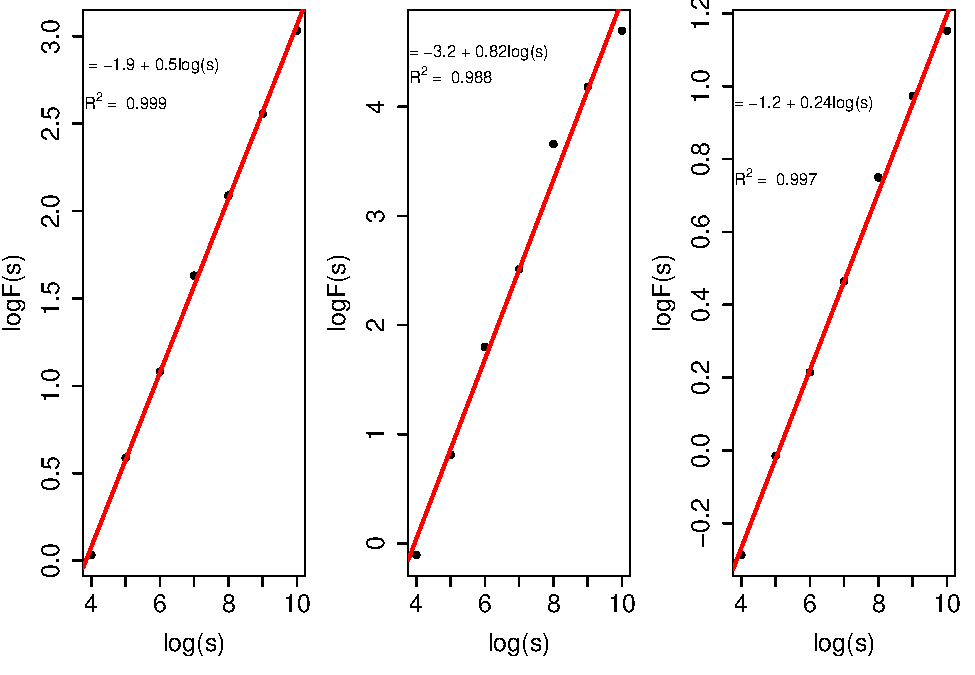
\includegraphics{fractal_regression_paper_brm_files/figure-latex/unnamed-chunk-3-1.pdf}

For an empirical example, we apply the \texttt{dfa()} function to the Human
Balance Dataset (Santos \& Duarte, 2016). This publicly available dataset includes
signals from a force platform that measures the center of pressure in
the x and y dimensions for 87 young adults (we exclude the older adults
from our analyses for simplicity). Trials lasted 60s. See original paper
for additional details on data processing (Santos \& Duarte, 2016). For the
empirical examples, we use two different time series featuring a
participant standing on a firm (rigid) surface with eyes open and a foam
(unstable) surface with eyes open. We chose this dataset because
postural sway data are known to exhibit interesting fractal dynamics
(Collins \& De Luca, 1993; Delignières, Torre, \& Bernard, 2011a; Delignières, Torre, \& Bernard, 2011b) and we can
systematically evaluate the data for all of the univariate and bivariate
analyses included in the package.

For center of pressure (COP) data, we take the first order differences
of each series using the \texttt{diff()} function as a rough approximation of
COP velocity. For the univariate analyses, we focus on analyses of the
COP data in the x dimension. Then, we define the appropriate scales for
the analyses using the same methods shown above, except we use a
\texttt{scale\ ratio\ =\ 1.1} for a higher density of points. Figure 2 shows the
results of these analyses.

\textbf{Figure 2}

\emph{Log scale-Log fluctuation plots for empirical differenced COPx time
series for rigid/firm (top) and unstable/foam (bottom) surfaces.}

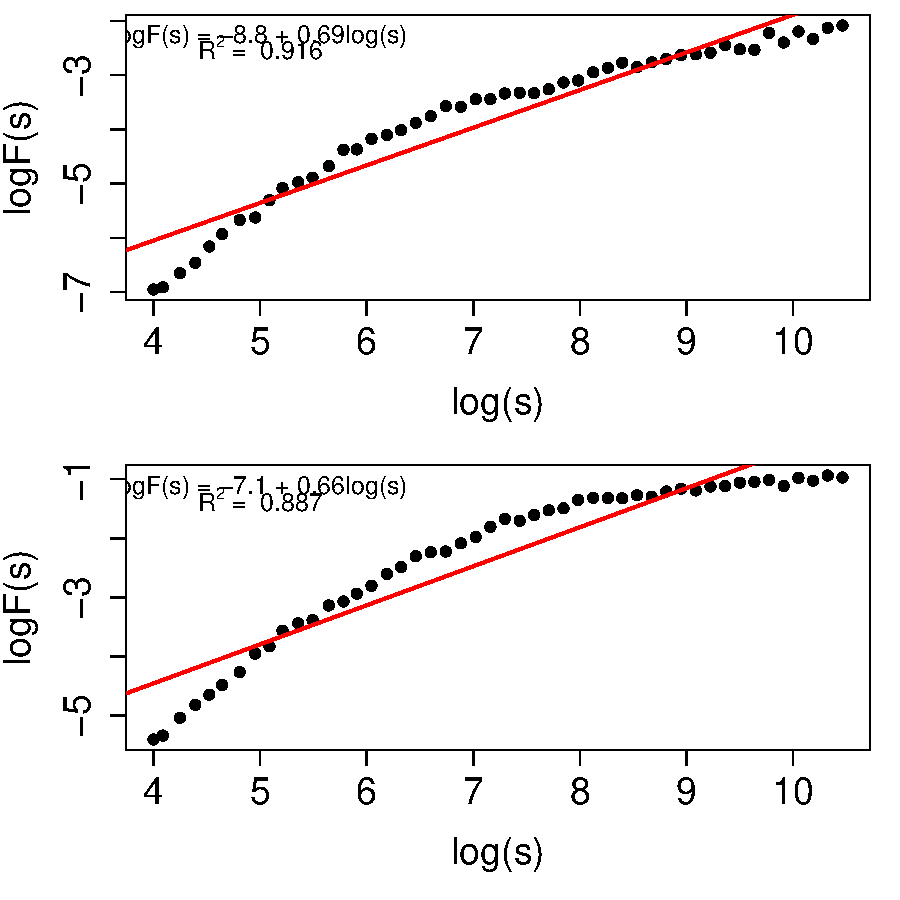
\includegraphics{fractal_regression_paper_brm_files/figure-latex/unnamed-chunk-5-1.pdf}

Importantly, regarding the question one can ask using DFA, we observe
from Figure 2, that long range correlations are positive and
approximately 0.69 -
0.66. However, from visual inspection of
these plots we observe that two slopes might fit better than one for
these time series; a phenomenon known as crossover points (Collins \& De Luca, 1993; Ge \& Leung, 2013). One common approach when such crossover points exist is to
recognize that the signal might be best characterized by two scaling
regions, before and after an inflection point. We provide an example of
how to check for where the break point is below using piece-wise
regression .

\begin{Shaded}
\begin{Highlighting}[]
\CommentTok{\# requires the segmented R package}

\NormalTok{dfa.mod }\OtherTok{\textless{}{-}} \FunctionTok{lm}\NormalTok{(log\_rms }\SpecialCharTok{\textasciitilde{}}\NormalTok{ log\_scales, }\AttributeTok{data =}\NormalTok{ open\_firm\_copx\_diff\_dfa)}

\NormalTok{seg }\OtherTok{\textless{}{-}} \FunctionTok{segmented}\NormalTok{(dfa.mod, }\AttributeTok{seg.Z =} \SpecialCharTok{\textasciitilde{}}\NormalTok{log\_scales)}
\end{Highlighting}
\end{Shaded}

\textbf{Figure 3}

\emph{Log scale-Log fluctuation plots for empirical differenced COPx time
series for rigid/firm surfaces with lines plotted for piece-wise
regression slopes}

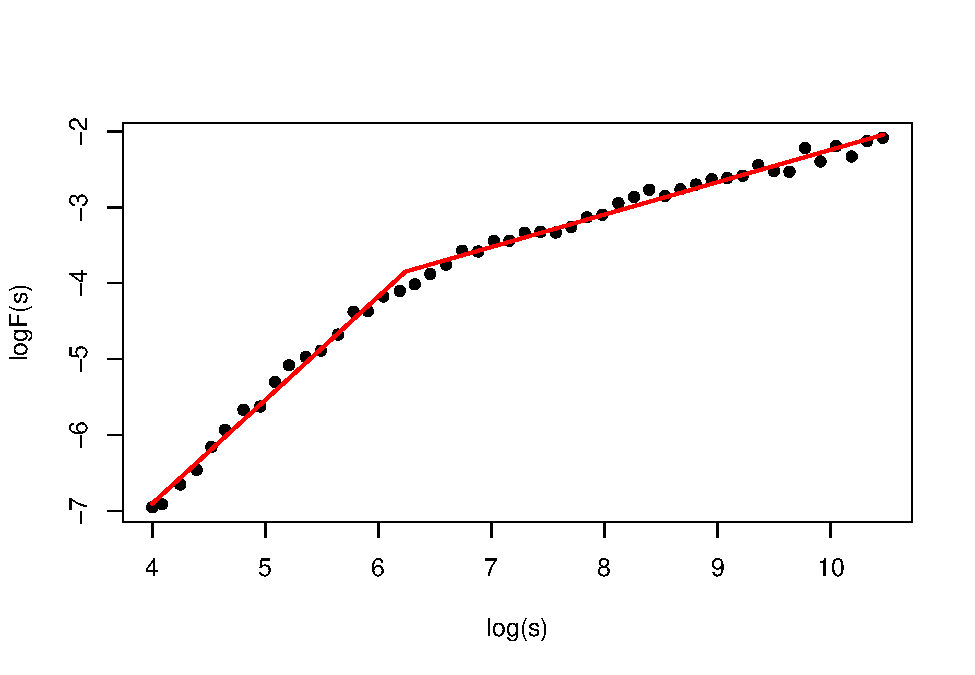
\includegraphics{fractal_regression_paper_brm_files/figure-latex/unnamed-chunk-7-1.pdf}

In the example above, we observe a crossover point at around the scale
size of log 6. And, from the results in Table 2 below, we observe that
there are two distinct scaling relationships corresponding to \(\alpha =\)
1.36 and \(\alpha =\) 0.43, respectively. This is a well known result in
the postural control literature such that short time scales exhibit a
persistent temporal correlation and that longer time scales exhibit an
anti-persistent correlation. More substantively, short time scale
dynamics correspond to periods of exploratory sway, whereas longer time
scales correspond to corrective movements that prevent exceeding the
base of support and falling (Collins \& De Luca, 1993; Delignières et al., 2011a; Delignières et al., 2011b).

\textbf{Table 2.}

\emph{Results from piece-wise regression analysis}

\begin{longtable}[]{@{}llllll@{}}
\caption{Results from piece-wise regression analysis}\tabularnewline
\toprule()
& Estimate & SE & \emph{t} & 95\% CI l & 95\% CI u \\
\midrule()
\endfirsthead
\toprule()
& Estimate & SE & \emph{t} & 95\% CI l & 95\% CI u \\
\midrule()
\endhead
Slope 1 & 1.36 & 0.03 & 40.66 & 1.30 & 0.40 \\
Slope 2 & 0.43 & 0.01 & 31.25 & 1.43 & 0.45 \\
\bottomrule()
\end{longtable}

\hypertarget{multifractal-detrended-fluctuation-analysis}{%
\subsubsection{Multifractal Detrended Fluctuation Analysis}\label{multifractal-detrended-fluctuation-analysis}}

Multifractal Detrended Fluctuation Analysis (MFDFA;
Kantelhardt et al. (2002)) is an extension of DFA
by generalizing the fluctuation function to a range of exponents of the
\(q\)th order. The key question that can be answered by MFDFA is: \emph{how
does the magnitude and direction of long range correlation change over
time within a single time series?} Like DFA, MFDFA entails splitting a
time series into several small bins (e.g., 16). In each bin, least
squares regression is fit and subtracted within each window. However,
the residuals are raised to a range of exponents \(q\) and averaged within
each window. So when \(q = 2\), MFDFA reduces to ordinary DFA. When
\(q >2\), relatively larger residuals are emphasized and when \(q < 2\),
relatively smaller residuals are emphasized. The rest of the DFA
algorithm is performed for each window and windows size for all values
of \(q\). We refer the reader to the work of Kelty-Stephens and
colleagues' (Kelty-Stephen et al., 2016) Figure
3 for a visualization of the algorithm, Appendix 1 of this paper for
fundemental equations, and Kantelhardt and colleagues' work
(Kantelhardt et al., 2002) for additional
mathematical description.

\hypertarget{mfdfa-examples}{%
\paragraph{MFDFA Examples}\label{mfdfa-examples}}

To demonstrate the use of \texttt{mfdfa()}, we work with data included in our
package (\texttt{fractaldata}), that was originally provided by
Ihlen (2012). It includes a white noise
time series, a monofractal time series, and a multifractal time series.
These data are shown below in Figure 4.

\textbf{Figure 4}

\emph{Time series from Ihlen (2012) corresponding to white noise,
monofractal, and multifractal series}

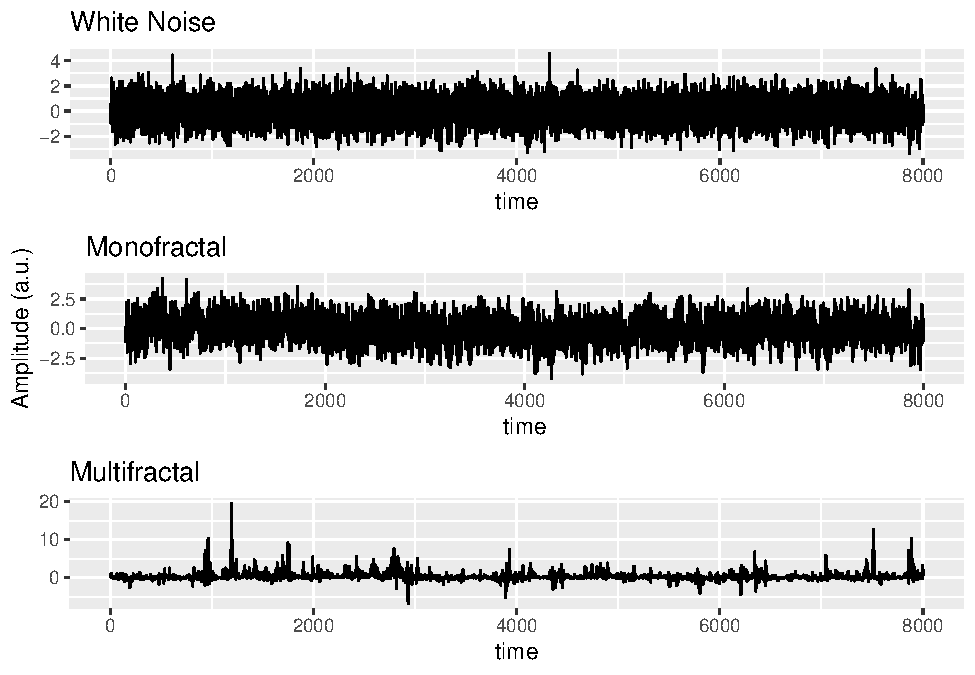
\includegraphics{fractal_regression_paper_brm_files/figure-latex/unnamed-chunk-9-1.pdf}

Performing MFDFA is straight forward with the \texttt{mfdfa()} function. As
shown in the example below, one enters the time series \texttt{x} to perform
the analysis on, the range of \texttt{q} order exponents to use, the \texttt{order} of
polynomial detrending, and the \texttt{scales} for the analysis. In this case,
we define our \texttt{scales} by choosing logarithmically spaced scales and we
select values of q from -5 to 5. Note here that the scale factor need
not be a power of two but should be evenly spaced in the logarithmic
domain by, for example, using different logarithm bases. We provide the
\texttt{logscale()} function to facilitate scale construction.

\begin{Shaded}
\begin{Highlighting}[]
\NormalTok{scales }\OtherTok{\textless{}{-}} \FunctionTok{logscale}\NormalTok{(}\AttributeTok{scale\_min =} \DecValTok{16}\NormalTok{,}\AttributeTok{scale\_max =} \DecValTok{1024}\NormalTok{,}\AttributeTok{scale\_ratio =} \FloatTok{1.1}\NormalTok{)}

\NormalTok{white.mf.dfa.out }\OtherTok{\textless{}{-}} \FunctionTok{mfdfa}\NormalTok{(}\AttributeTok{x =}\NormalTok{ fractaldata}\SpecialCharTok{$}\NormalTok{whitenoise, }\AttributeTok{q =} \FunctionTok{c}\NormalTok{(}\SpecialCharTok{{-}}\DecValTok{5}\SpecialCharTok{:}\DecValTok{5}\NormalTok{), }
\AttributeTok{order =} \DecValTok{1}\NormalTok{, }\AttributeTok{scales=}\NormalTok{scales, }\AttributeTok{scale\_ratio=}\FloatTok{1.1}\NormalTok{)}

\NormalTok{mono.mf.dfa.out }\OtherTok{\textless{}{-}} \FunctionTok{mfdfa}\NormalTok{(}\AttributeTok{x =}\NormalTok{ fractaldata}\SpecialCharTok{$}\NormalTok{monofractal, }\AttributeTok{q =} \FunctionTok{c}\NormalTok{(}\SpecialCharTok{{-}}\DecValTok{5}\SpecialCharTok{:}\DecValTok{5}\NormalTok{),}
\AttributeTok{order =} \DecValTok{1}\NormalTok{,  }\AttributeTok{scales=}\NormalTok{scales, }\AttributeTok{scale\_ratio=}\FloatTok{1.1}\NormalTok{)}

\NormalTok{multi.mf.dfa.out }\OtherTok{\textless{}{-}} \FunctionTok{mfdfa}\NormalTok{(}\AttributeTok{x =}\NormalTok{ fractaldata}\SpecialCharTok{$}\NormalTok{multifractal, }\AttributeTok{q =} \FunctionTok{c}\NormalTok{(}\SpecialCharTok{{-}}\DecValTok{5}\SpecialCharTok{:}\DecValTok{5}\NormalTok{),}
\AttributeTok{order =} \DecValTok{1}\NormalTok{,  }\AttributeTok{scales=}\NormalTok{scales, }\AttributeTok{scale\_ratio=}\FloatTok{1.1}\NormalTok{)}
\end{Highlighting}
\end{Shaded}

A common way to understand if there is evidence of multifractality is to
examine a plot showing the slopes of the \texttt{log\_fq} at the \texttt{log\_scale}
values. If all the lines have the same slope, that provides evidence of
monofractality. If there are distinct slopes, then there is evidence of
multifractality. It's also important to check here that the slopes of
\texttt{log\_scale} and \texttt{log\_fq} are approximately linear, thus implying that
they are scale invariant. If not, then it could be the case that a
higher order polynomial detrending is appropriate (see Kantelhardt et
al., 2001). Figure 5, in the top left quadrants, shows what we would
expect for a monofractal and multifractal signal. In other words, the
monofractal signal shows a consistent slope, whereas the multifractal
signal shows variability in the slopes. Importantly, Figure 5, using our
\texttt{mfdfa.plot()} function, shows various aspects of mfdfa for each value
of q (each with its own color) and includes panels that show the
log(scale)-log(Fluctuation) plots like in the DFA plots (top left), the
slopes of those lines as the q-order Hurst exponents \(H(q)\) for each
value of q (top right), the mass exponents (\(\tau(q)\)) for each value of
q (bottom left), and the multifractal spectrum showing q-order
singularity values (h) for their dimension (D(h) for each value of q
(bottom right). See Ihlen (2012) for additional details of these
metrics.

\textbf{Figure 5}

\emph{Mfdfa.plots for mono-(top) and multifractal series (bottom)}

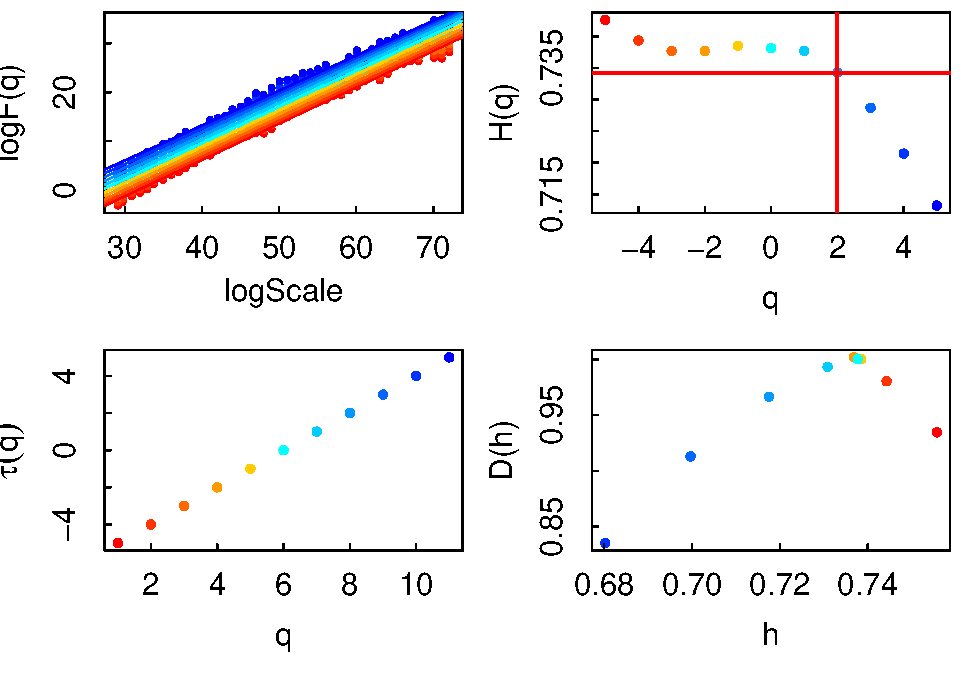
\includegraphics{fractal_regression_paper_brm_files/figure-latex/unnamed-chunk-11-1.pdf} 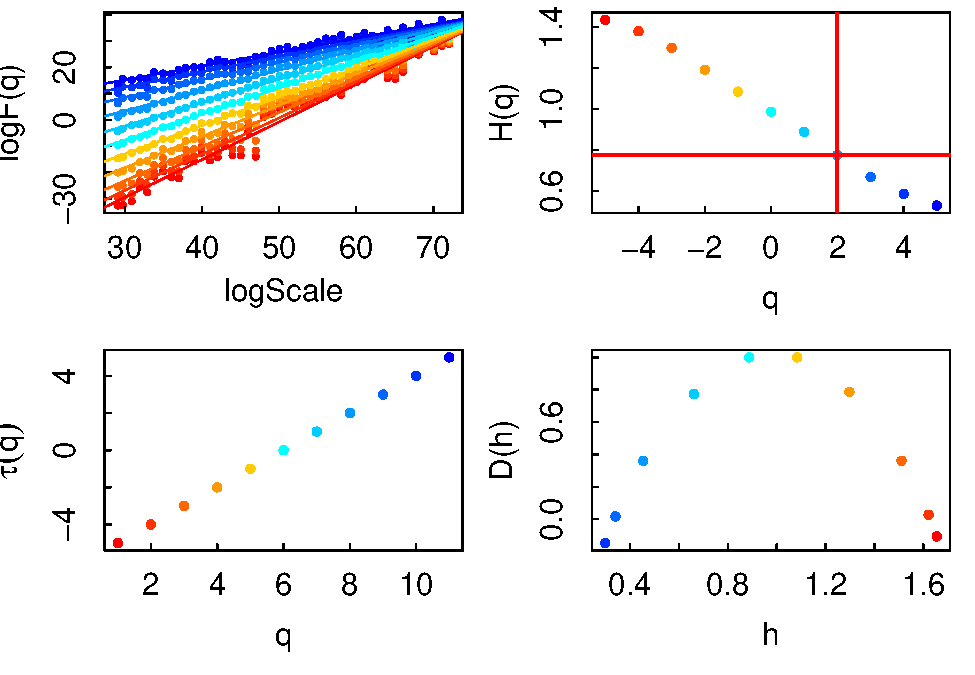
\includegraphics{fractal_regression_paper_brm_files/figure-latex/unnamed-chunk-11-2.pdf}

A common metric for comparing multifractal spectra is to calculate the
width (\(W\)) as \(h_{max} - h_{min}\). Let's do this to compare the
monofractal and multifractal time series. We observe in this case that
for the monofractal signal \(W_{mono} =\)
0.08 and \(W_{multi} =\)
1.36. If we compare the
spectra for the mono- and multifractal signals above (bottom right of
both plots), we observe this clear difference in the widths of the
multifractal spectra for the signals.

For our empirical analysis, we again turn to the postural data. We set
our parameters appropriate for the data and run \texttt{mfdfa()} on the
differenced COPx data for the firm and foam surfaces. Figure 6 shows the
plots for these analyses. In particular, we observe for both surfaces
that the q-order Hurst exponents range from
0.57 -
1.03,
all suggesting positive long-range correlations with a weakening of the
strength at larger values of q (i.e., trending towards white noise). The
multifractal spectrum widths of the two surfaces were also similar,
\(W_{foam} =\)
0.69
and \(W_{firm} =\)
0.70.

\textbf{Figure 6}

\emph{Mfdfa.plots for the firm (top) and foam surfaces (bottom)}

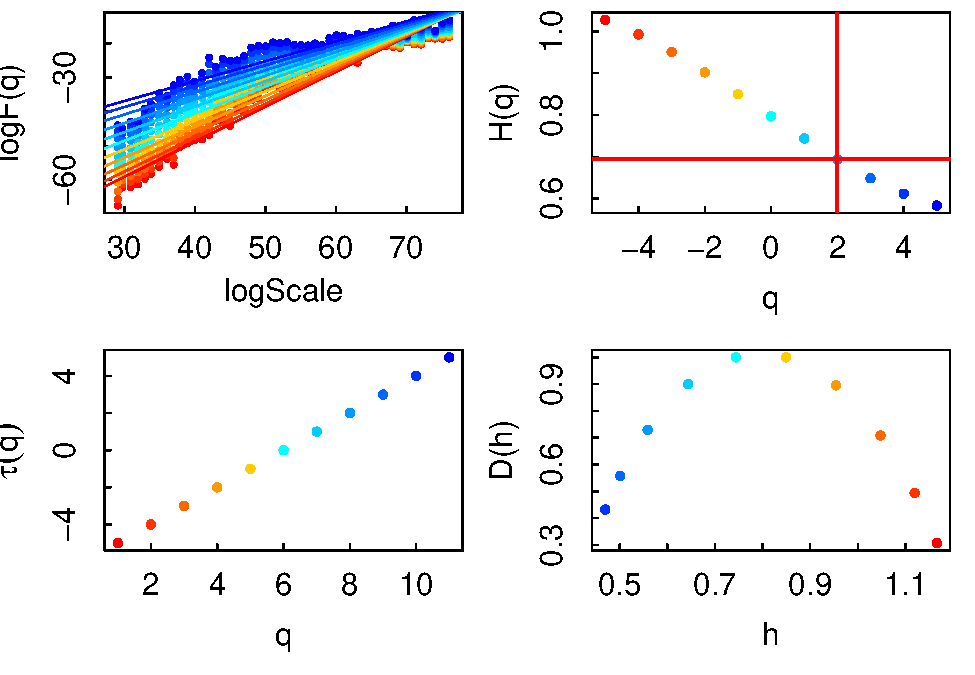
\includegraphics{fractal_regression_paper_brm_files/figure-latex/unnamed-chunk-13-1.pdf} 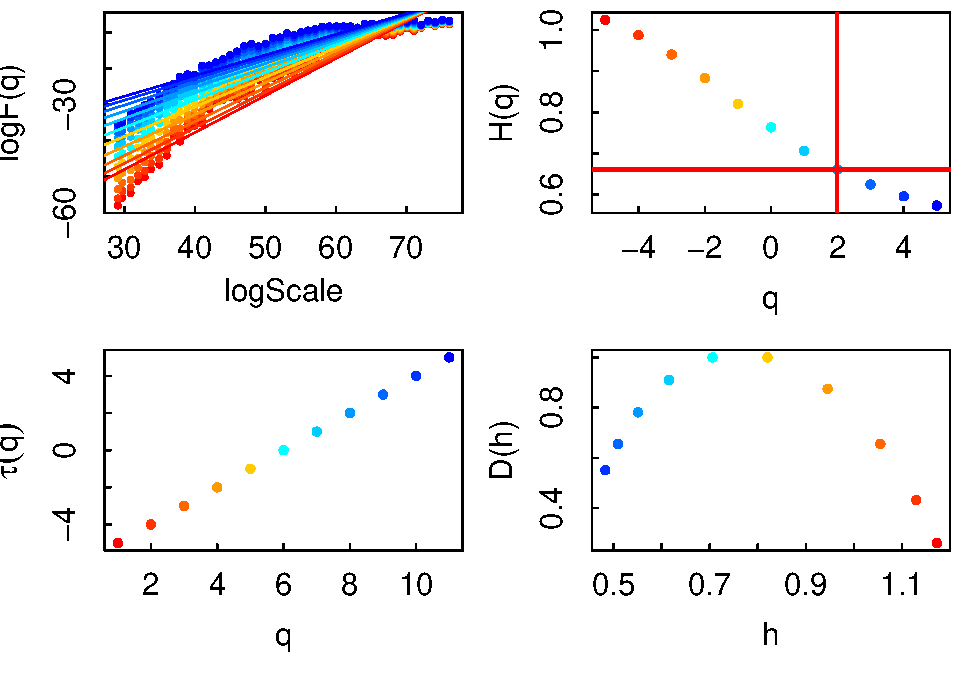
\includegraphics{fractal_regression_paper_brm_files/figure-latex/unnamed-chunk-13-2.pdf}

\hypertarget{bivariate-methods}{%
\subsection{Bivariate Methods}\label{bivariate-methods}}

\hypertarget{detrended-cross-correlation-analysis}{%
\subsubsection{Detrended Cross-Correlation Analysis}\label{detrended-cross-correlation-analysis}}

Detrended Cross-Correlation Analysis (DCCA
(Podobnik \& Stanley, 2008; Zebende, 2011) is a bivariate extension of
the DFA algorithm generalizing it to a correlational case between two
time series that may be non-stationary. The key questions that can be
asked with it are: a) \emph{How does the correlation between two time series
change as a function of scale?} and b) \emph{What is/are the dominant (time)
scale(s) of coordination?} Such decisions are based on a predetermined
threshold such as a conventional statistical significance as we
demonstrate below. Researchers may also select other criteria
appropriate for their research area.The DCCA algorithm is a direct
generalization of the DFA algorithm but applied to two concomitantly
measured time series, say \emph{x} and \emph{y}. As in DFA, time series are split
into multiple bins and detrended using least squares regression.
Separate regressions are performed for \emph{x} and \emph{y}. Within each bin,
three quantities are estimated, the average squared residual of \emph{x,} the
average squared residual of \emph{y}, and the average cross product (i.e.,
the covariance) between the residuals for \emph{x} and the residuals for \emph{y}.
Each of those quantities is averaged across all bins of a given size.
After taking the squared residual for \emph{x} and \emph{y}, we obtain scale-wise
equivalents of covariance \(F_{xy}(s)\) and standard deviations for \emph{x}
\(F_x(s)\) and \emph{y} \(F_y(s)\). The use of \(F\) to designate these quantities
derives from originating literature (Kristoufek, 2015b; Likens, Amazeen, West, \& Gibbons, 2019b).
Thus, the scale-wise regression coefficient, the estimand of DCCA, is
the following quotient:

\[\rho(s)=\frac{F_{xy}(s)}{F_x(s)F_y(s)}\]

Simplified, like DFA, the key metric is \(\alpha\), but in DCCA, one
estimates the scale-specific, detrended cross-correlation coefficient
\(\rho(s)\) for the pair of time series.

\hypertarget{dcca-examples}{%
\paragraph{DCCA Examples}\label{dcca-examples}}

To demonstrate the use of \texttt{dcca()}, we used the \texttt{mc\_arfima()} function
from our package to simulate two time series with known properties.
Specifically, we use the multicorrelated ARFIMA examples from
Kristoufek's work (Kristoufek, 2013). In
this case, we use the parameters from Kristoufek (2013) for Model 1 (p.
6,487), that generates two time series of length 10,000 that exhibit
long range correlations (LRC) as well as long range cross-correlations
(LRCC). The code for simulating these two time series is shown below.
Additionally, Figure 7, shown below, visualizes a subset of these time
series.

\begin{Shaded}
\begin{Highlighting}[]
\FunctionTok{set.seed}\NormalTok{(}\DecValTok{987345757}\NormalTok{)}

\NormalTok{sim1 }\OtherTok{\textless{}{-}} \FunctionTok{mc\_ARFIMA}\NormalTok{(}\AttributeTok{process=}\StringTok{"Mixed\_ARFIMA\_ARFIMA"}\NormalTok{, }\AttributeTok{alpha =} \FloatTok{0.2}\NormalTok{, }
\AttributeTok{beta =} \DecValTok{1}\NormalTok{, }\AttributeTok{gamma =} \DecValTok{1}\NormalTok{, }\AttributeTok{delta =} \FloatTok{0.2}\NormalTok{, }\AttributeTok{n =} \DecValTok{10000}\NormalTok{, }\AttributeTok{d1 =} \FloatTok{0.4}\NormalTok{, }\AttributeTok{d2 =} \FloatTok{0.3}\NormalTok{, }
\AttributeTok{d3 =} \FloatTok{0.3}\NormalTok{, }\AttributeTok{d4=}\FloatTok{0.4}\NormalTok{, }\AttributeTok{rho=}\FloatTok{0.9}\NormalTok{)}
\end{Highlighting}
\end{Shaded}

\textbf{Figure 7}

\emph{Subset of two time series exhibiting long range correlation and long
range cross-correlation}

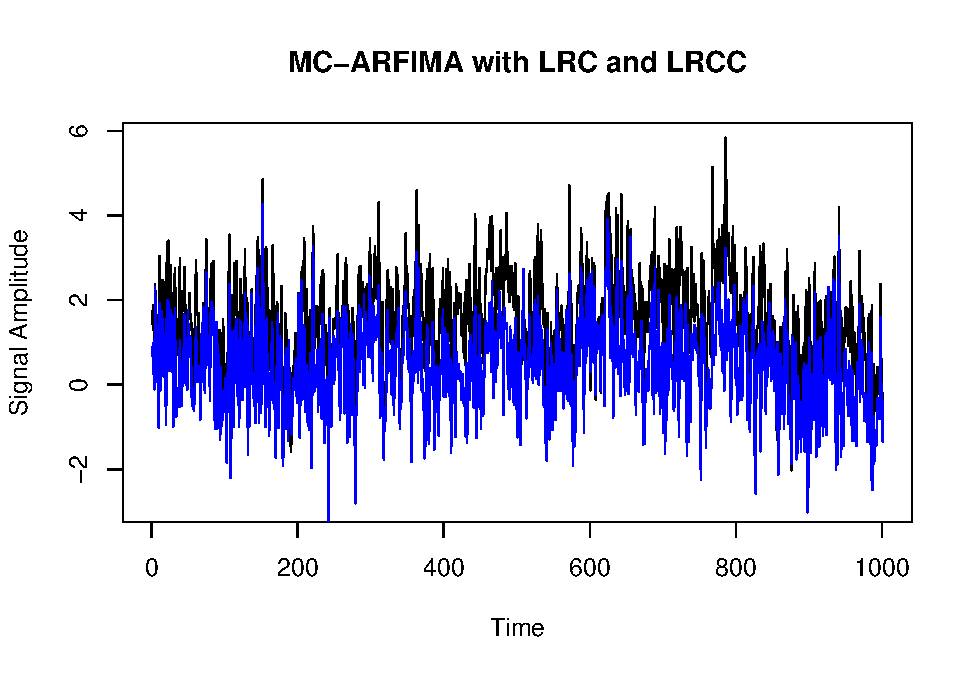
\includegraphics{fractal_regression_paper_brm_files/figure-latex/unnamed-chunk-15-1.pdf}

As can be seen in Figure 7, the simulated time series, although quite
noisy, appear to covary over time with similar trends. To perform the
\texttt{dcca()} on these time series, we use the code below, where we first
define the \texttt{scales} using the \texttt{logscale()} function described earlier
along with the \texttt{dcca()} function itself.

\begin{Shaded}
\begin{Highlighting}[]
\NormalTok{scales }\OtherTok{\textless{}{-}} \FunctionTok{logscale}\NormalTok{(}\AttributeTok{scale\_min =} \DecValTok{10}\NormalTok{, }\AttributeTok{scale\_max =} \DecValTok{1000}\NormalTok{, }\AttributeTok{scale\_ratio =} \FloatTok{1.1}\NormalTok{)}

\NormalTok{dcca.out.arfima }\OtherTok{\textless{}{-}} \FunctionTok{dcca}\NormalTok{(sim1[,}\DecValTok{1}\NormalTok{], sim1[,}\DecValTok{2}\NormalTok{], }\AttributeTok{order =} \DecValTok{1}\NormalTok{, }\AttributeTok{scales =}\NormalTok{ scales)}
\end{Highlighting}
\end{Shaded}

Next, we visualize the output of DCCA in Figure 8. We observe that, as
expected, the correlation between the MC-ARFIMA processes are
consistently high (all \(\rho\)'s \(> .8\)) and continue to be high at
increasing time scales.

\textbf{Figure 8}

\emph{DCCA output for long range correlation and long range
cross-correlation}

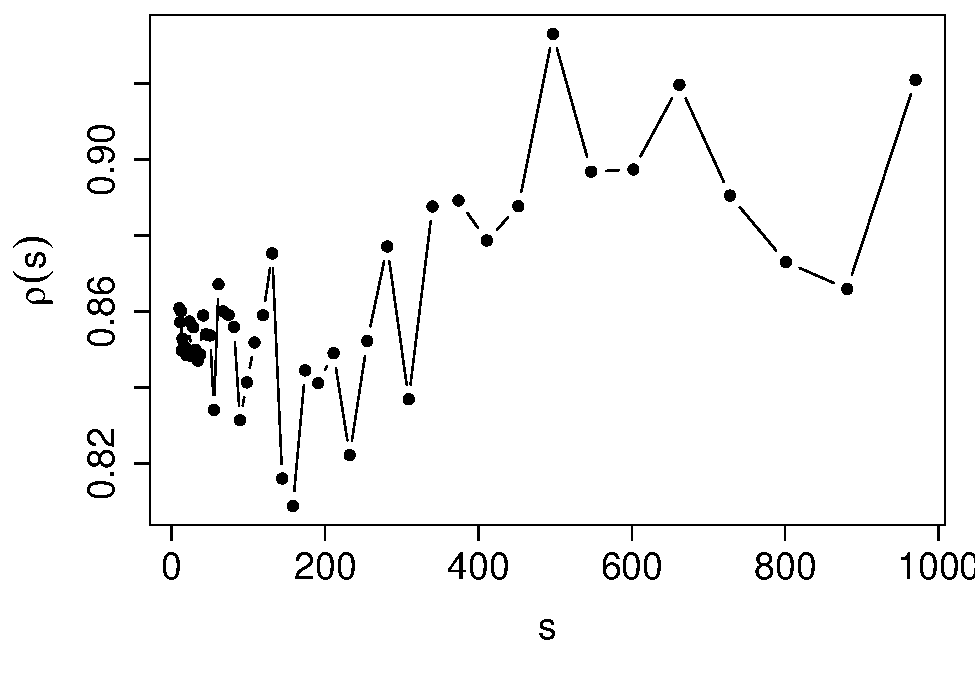
\includegraphics{fractal_regression_paper_brm_files/figure-latex/unnamed-chunk-17-1.pdf}

Figure 8 is difficult to interpret on its own. To address this, we
demonstrate an additional plot and analysis feature of \texttt{dcca()} by
modifying the above code as shown below \texttt{ci\ =\ TRUE}. Loess smoothing can
also be applied to both \(\rho(s)\) and its confidence intervals using
\texttt{loess.rho\ =\ TRUE} and \texttt{loess.ci\ =\ TRUE}. Those latter options are
useful for reducing the impact of increasing variance on estimates of
\(\rho(s)\) at large scales (Likens et al., 2019b). Note though that a much larger
set of calculations takes place and may take several seconds up to
several minutes (for long time series) to complete. This method is shown
in Figure 9. Importantly, it shows us that there is evidence of long
range cross-correlations as there \(\rho(s)\) for all scales are outside
of the surrogate confidence interval.

\textbf{Figure 9}

\emph{DCCA output for long range correlation and long range cross-correlation
with Loess smoothing on estimates and a surrogate confidence interval}

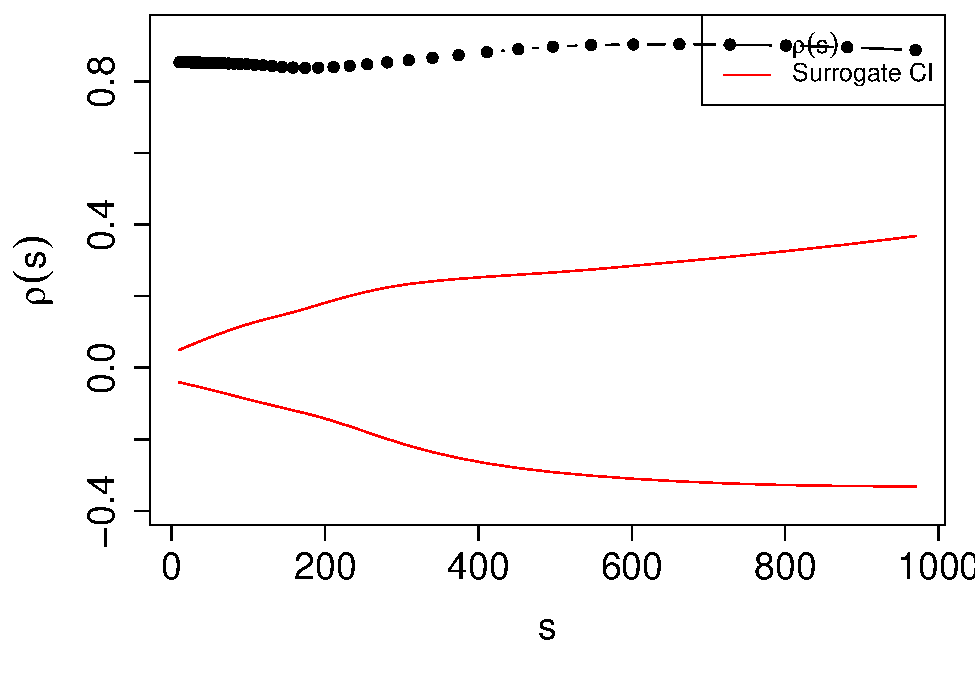
\includegraphics{fractal_regression_paper_brm_files/figure-latex/unnamed-chunk-18-1.pdf}

As a point of comparison, we can generate a time series in contrast with
this that exhibits processes with LRC and short-range cross-correlation
(SRCC) using the code below. In contrast to the previous DCCA analysis,
Figure 10 shows a signal that begins with a high cross-correlation
(\(\rho\)'s \(\approx .6\)), but that begins to deviate and trend
substantially lower at increasing scale sizes with \(\rho\) entering the
confidence interval containing 0. In fact, based on the plotted
confidence intervals, the correlation between the two series becomes
non-significant from a conventional standpoint.

\textbf{Figure 10}

\emph{DCCA output for long range correlation and short range
cross-correlation including smoothing and a surrogate confidence
interval}

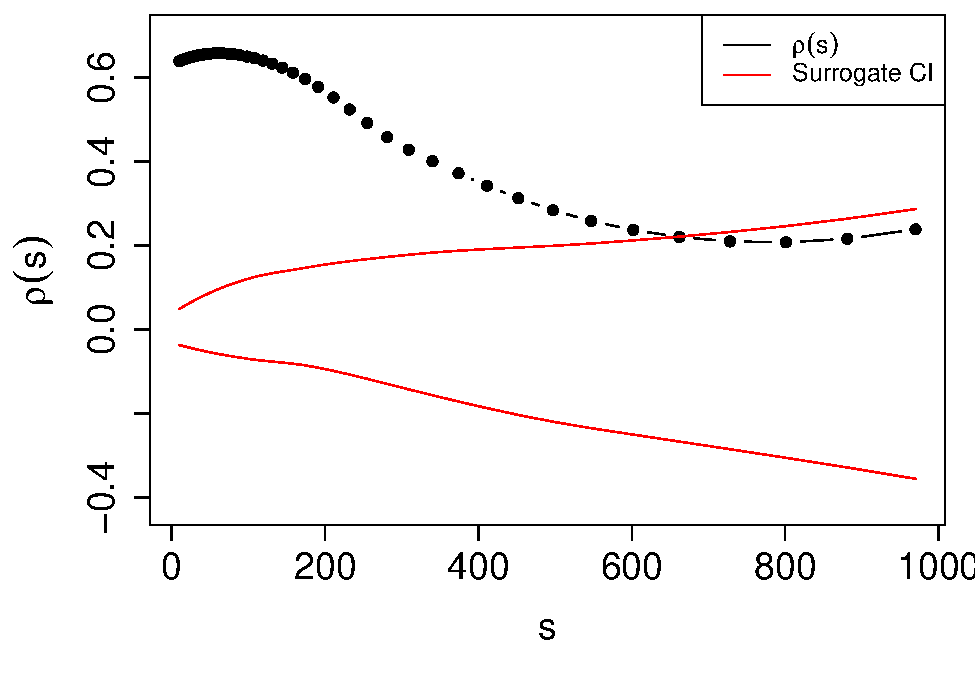
\includegraphics{fractal_regression_paper_brm_files/figure-latex/unnamed-chunk-20-1.pdf}

Turning next to the empirical balance data, we apply DCCA to the
differenced COPx \emph{and} COPy data for the firm and foam platforms. We
again set appropriate values for \texttt{scales} and apply the \texttt{dcca()}
function to the pair of time series.

\textbf{Figure 11}

\emph{DCCA output for empirical COPx and COPy balance data for the eyes open
while standing on the firm surface (top) and foam surface (bottom)}

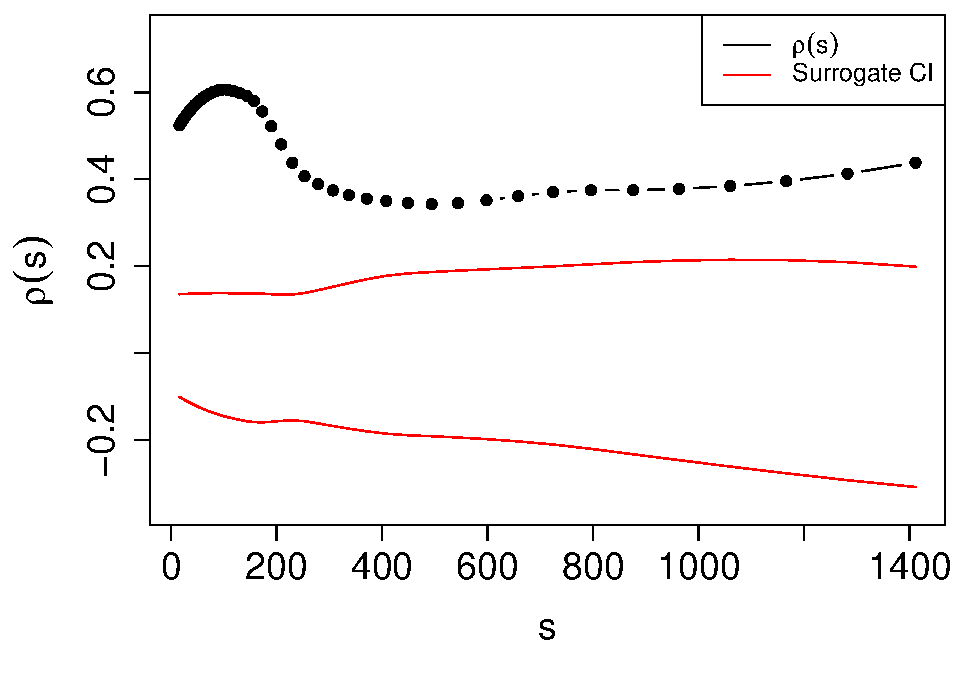
\includegraphics{fractal_regression_paper_brm_files/figure-latex/unnamed-chunk-22-1.pdf} 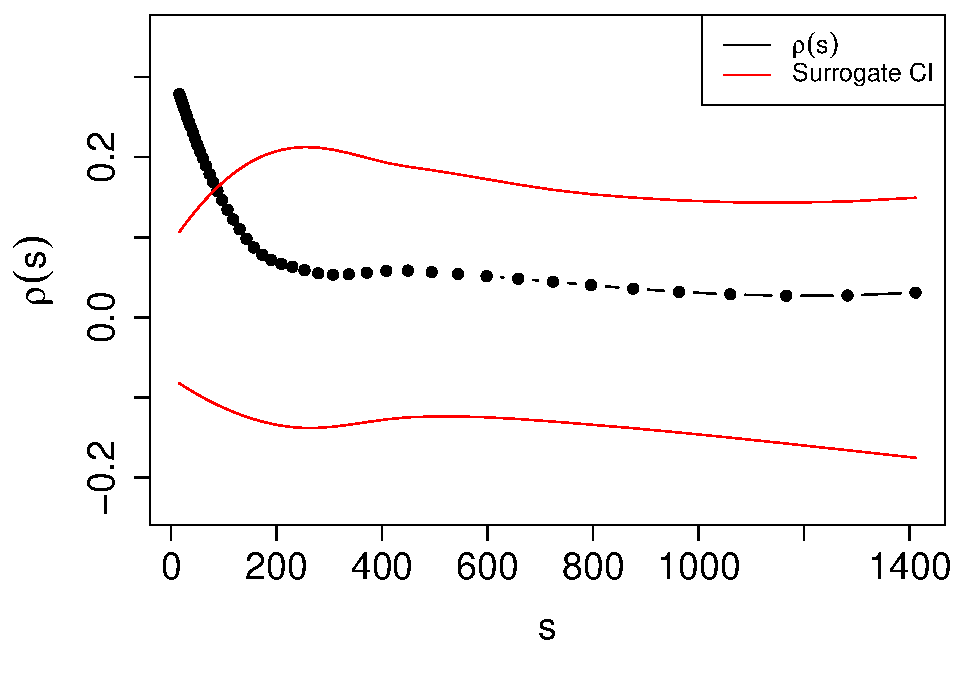
\includegraphics{fractal_regression_paper_brm_files/figure-latex/unnamed-chunk-22-2.pdf}

In examining the output from these analyses, Figure 11 shows a clear
difference between the two conditions. First, in the firm platform
example, the \(\rho(s)\) values reach an order of magnitude greater than
in the foam condition with the max \(\rho(s)\) =
0.73 compared to
0.35 for the foam condition. Second, we
observe for the foam example, that the time scale of maximum correlation
is 73,
which is a larger time scale when compared to the foam example, which
had a maximum correlation at scale
16. Third,
the pattern of change in correlation across scales is slightly
different. The firm example is higher overall; it starts relatively low
at very small time scales before a rapid increase and then steady
decrease before stabilizing at increasingly larger scales. By contrast,
the foam example has relatively lower overall correlation values, the
smallest scale is the highest followed by a steady decrease and then
also stabilizing at larger scales. Lastly, we can also derive
statistical conclusions because, in the firm condition, the two series
are correlated at all scales, whereas the series are only correlated
beyond chance at the smaller scales in the foam condition.

\hypertarget{multiscale-regression-analysis}{%
\subsubsection{Multiscale Regression Analysis}\label{multiscale-regression-analysis}}

Multiscale regression analysis (MRA) is a further generalization of DCCA
that brings the analyses into a predictive, regression framework
(Kristoufek, 2015b). The key questions that can be answered by it are: a)
\emph{How does the influence of one time series on another time series change
as a function of scale?} and b) \emph{What is/are the dominant (time)
scale(s) of influence of one time series on another time series?} The
algorithm is largely the same as DCCA, with a key difference being that
instead of estimating scale-wise symmetric correlation coefficients,
leveraging methods of Ordinary Least Squares (OLS) regression,
asymmetric \(\beta\) coefficients are estimated (Kristoufek, 2015b; Likens et al., 2019b) according to the following equation:

\[
\beta(s)=\frac{F_{xy}(s)}{F^2_x(s)}
\]

The \(\beta(s)\) equation differs from the \(\rho(s)\) equation only in the
denominator where \(F^2_x(s)\) is the average squared residual at each
scale and \(F_xy(s)\) is still the scale-wise covariance.

\hypertarget{mra-examples}{%
\paragraph{MRA Examples}\label{mra-examples}}

Considering the LRC and LRCC simulations used for DCCA, we can examine
whether the scale-wise fluctuations of one variable can predict the
scale-wise fluctuations of the other using \texttt{mra()}. As with a
traditional regression approach, we will use one of our variables as our
predictor (\(x_t\)) and the other as our outcome (\(y_t\)). In the example
below, we again first define our logarithmically spaced scales. We then
apply the \texttt{mra()} function to the two simulated time series. In this
case, it's important to specify which is variable is \texttt{x} (the predictor)
and which is \texttt{y} (the outcome).

\begin{Shaded}
\begin{Highlighting}[]
\NormalTok{scales }\OtherTok{\textless{}{-}} \FunctionTok{logscale}\NormalTok{(}\AttributeTok{scale\_min =} \DecValTok{10}\NormalTok{, }\AttributeTok{scale\_max =} \DecValTok{1000}\NormalTok{, }\AttributeTok{scale\_ratio =} \FloatTok{1.1}\NormalTok{)}

\NormalTok{mra.out }\OtherTok{\textless{}{-}} \FunctionTok{mra}\NormalTok{(}\AttributeTok{x =}\NormalTok{ sim1[,}\DecValTok{1}\NormalTok{], }\AttributeTok{y =}\NormalTok{ sim1[,}\DecValTok{2}\NormalTok{], }\AttributeTok{order =} \DecValTok{1}\NormalTok{, }\AttributeTok{scales =}\NormalTok{ scales)}
\end{Highlighting}
\end{Shaded}

We can then visualize these results as shown below in Figure 12.
Generally, we observe that the \(\beta\) coefficients are relatively
stable at increasing time scales with a general, perhaps quadratically
increasing trend. Here it is also important to investigate the change in
\(R^2\) as well as the \(t\)-values. Below we see that the \(R^2\) is quite
high at most of the time scales with \(R^2_{min} =\)
0.67 and \(R^2_{max} =\)
1.85 and all \(\beta(s)\) exceed the confidence
intervals, implying conventional statistical significance. So between
these two component ARFIMA processes, the output of MRA shows that much
of the scale specific variance in \(y_t\) is explained and predicted by
\(x_t\).

\textbf{Figure 12}

\emph{MRA output for long range correlation and long range cross-correlation}

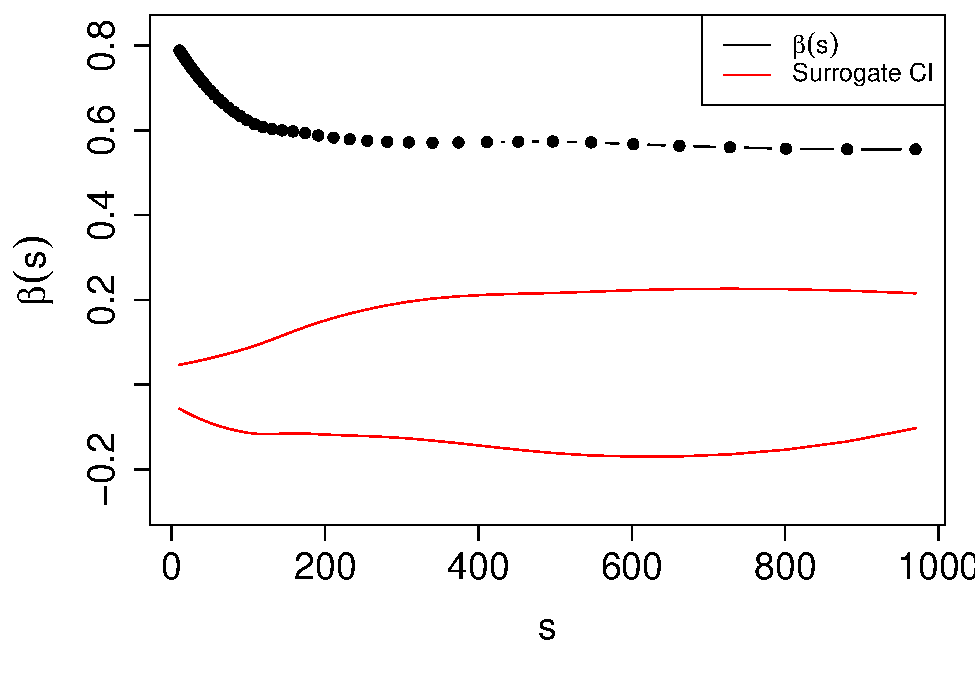
\includegraphics{fractal_regression_paper_brm_files/figure-latex/unnamed-chunk-24-1.pdf}

Turning next to the empirical balance data, we can determine whether
postural adjustments in the COPx are predictive of adjustments in COPy,
and vice versa. This means that we use the \texttt{mra()} function two times
and reverse the order of entry for the x and y arguments to allow for
determining the degree to which each signal can predict the other across
scales. In Figure 13 below, we see the resulting \(\beta\)'s we observed
for the the balance data on the firm surface. Notably, the COPx
predicting COPy (max \(\beta\) = 0.19) has
noticeably smaller \(\beta\) values compared to COPy predicting COPx (max
\(\beta\) = 3.25). Notice as well how Figure 13
(bottom), where adjustments in the y dimension are predicting
adjustments in the x dimension, resembles the DCCA plot for this
analysis (see Figure 11). Given the asymmetry in the magnitude of the
\(\beta\)s, this example suggests that postural adjustments in the y
dimension appear to be driving changes in the x dimension. And, there is
a clear time scale where this relationship is strongest at scales =
55, implying a
dominant mode of coordination between mediolateral and anterioposterior
control processes.

\textbf{Figure 13}

\emph{MRA output for balance data on foam surface with COPx predicting COPy
(top) and COPy predicting COPx (bottom).}

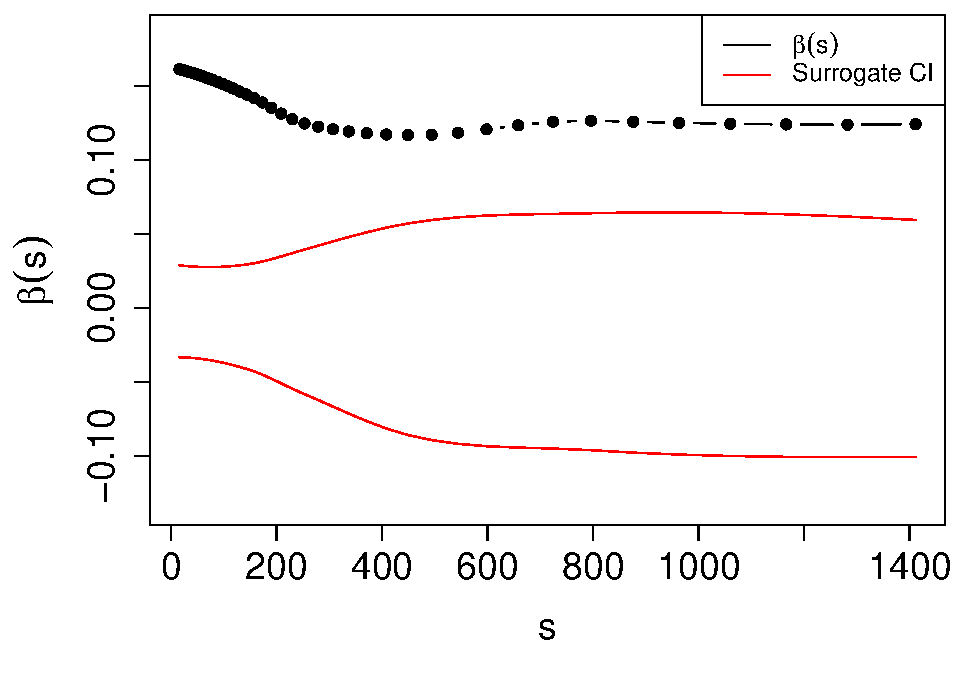
\includegraphics{fractal_regression_paper_brm_files/figure-latex/unnamed-chunk-26-1.pdf} 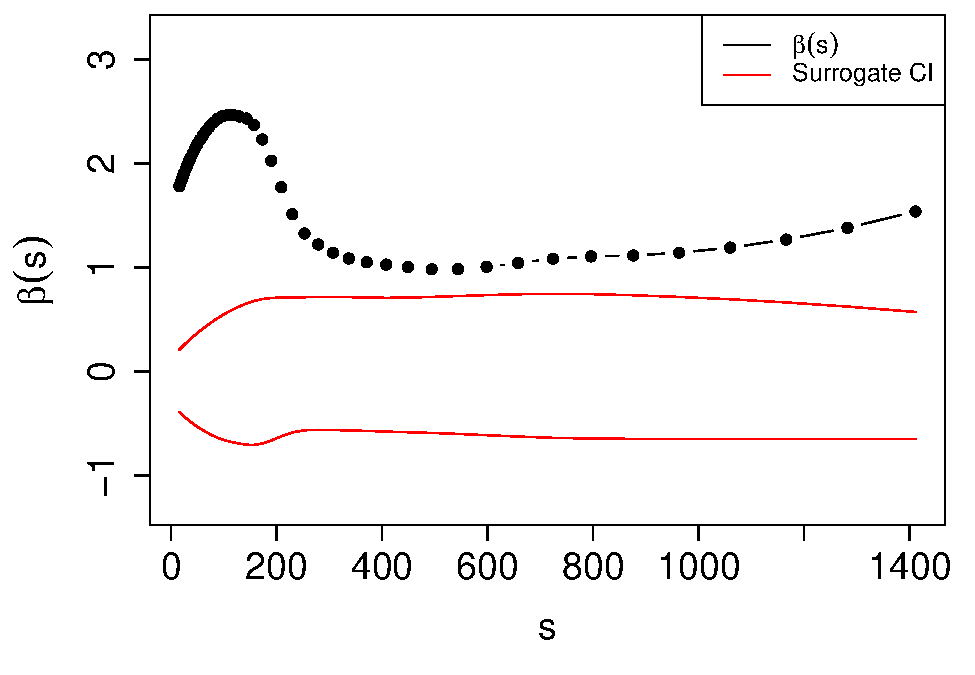
\includegraphics{fractal_regression_paper_brm_files/figure-latex/unnamed-chunk-26-2.pdf}

\hypertarget{surrogate-methods}{%
\subsection{Surrogate Methods}\label{surrogate-methods}}

In all of the above methods, one gets either a single estimate of a
parameter (e.g., \(\alpha\)) or a range of estimates (e.g., \(\rho(s)\),
\(\beta(s)\)). While those estimates are meaningful in and of themselves,
it is common practice to perform some form of null hypothesis test
regarding the estimate(s). These are generally referred to as surrogate
methods (Kantz \& Schreiber, 2003). We present several options here that could be
ranked in terms of increasing levels of rigor: randomized surrogates,
iterative amplitude adjusted Fourier transformed (IAAFT) surrogates, and
model-based surrogates.

\hypertarget{randomized-surrogates}{%
\subsubsection{Randomized Surrogates}\label{randomized-surrogates}}

Randomized surrogates generally involve randomly shuffling the order of
values of a time series. The idea is generally that the temporal
structure is destroyed, yet the other features of the time series still
exist (Kantelhardt et al., 2002). The confidence
intervals for all of our plotting methods use this technique. Note that
additional options exist along these lines (see for example
(Dumas, Nadel, Soussignan, Martinerie, \& Garnero, 2010)). The key comparison here
would be to compare the estimates extracted from a given analysis (e.g.,
DFA) on the observed sample of data with the estimates derived from an
equally sized sample of the surrogate series (Kantz \& Schreiber, 2003; Moulder, Boker, Ramseyer, \& Tschacher, 2018; Wiltshire, Steffensen, \& Fiore, 2019).

\begin{Shaded}
\begin{Highlighting}[]
\NormalTok{rand.surr }\OtherTok{\textless{}{-}}\NormalTok{ permute}\SpecialCharTok{::}\FunctionTok{shuffle}\NormalTok{(pink.noise)}

\NormalTok{dfa.rand.surr }\OtherTok{\textless{}{-}} \FunctionTok{dfa}\NormalTok{(}\AttributeTok{x =}\NormalTok{ rand.surr, }\AttributeTok{order =} \DecValTok{1}\NormalTok{, }\AttributeTok{verbose =} \DecValTok{1}\NormalTok{,}
\AttributeTok{scales =}\NormalTok{ scales, }\AttributeTok{scale\_ratio =} \FloatTok{1.1}\NormalTok{)}
\end{Highlighting}
\end{Shaded}

Randomizing the pink noise time series, which originally exhibited long
range correlation (\(\alpha\) = 0.82), and performing DFA on
it, now provides an estimate of \(\alpha\) = 0.55,
which is consistent with a random or white noise process. These values
are clearly different, however, performing inferential statistics on a
sample of observed estimates compared to surrogate estimates would
provide compelling evidence that the temporal dynamics suggested by the
observed estimates are different than those derived from a random
process.

\hypertarget{iterative-amplitude-adjusted-fourier-transform-surrogates-iaaft}{%
\subsubsection{Iterative Amplitude-Adjusted Fourier Transform Surrogates (IAAFT)}\label{iterative-amplitude-adjusted-fourier-transform-surrogates-iaaft}}

The IAAFT algorithm was originally developed as a way to discern whether
nonlinearity is a feasible explanation for time series patterns
(Schreiber \& Schmitz, 1996). More recently, it was proposed as a technique to
determine if multifractal indices suggest interaction across scales
(Ihlen \& Vereijken, 2010). Like with randomized shuffling, estimates derived from
IAAFT surrogates should be also be different from the estimates derived
from the empirical time series. Although in this case, the comparison is
typically made between the multifractal spectra of the observed time
series, and the typical spectrum derived empirically from a set of IAAFT
surrogate series.

In the code below, we provide an example for generating IAAFT surrogates
using the \texttt{iaafft()} function in the package. One enters the \texttt{signal},
which is the observed time series, and \texttt{N}, the number of surrogates to
generate. There are a number of options here, but a common number of
surrogates is 19 (Kantz \& Schreiber, 2003), which allows one to establish a 95\%
confidence interval. In practice, surrogates are generated from each
observed time series. Here we illustrate the process using only a single
time series: the multifractal signal used previously in the MFDFA
example. Then we use the same parameters for the \texttt{mfdfa()} function, but
apply it to all of the IAAFFT surrogates. Note also that surrogate
analysis is `built-in' to our plot functions within the package as well
with options to return the relevant empirically derived confidence
intervals.

\begin{Shaded}
\begin{Highlighting}[]
\NormalTok{iaafft.surr }\OtherTok{\textless{}{-}} \FunctionTok{iaafft}\NormalTok{(fractaldata}\SpecialCharTok{$}\NormalTok{multifractal, }\AttributeTok{N =} \DecValTok{19}\NormalTok{)}

\NormalTok{iaafft.surr.out }\OtherTok{\textless{}{-}} \FunctionTok{apply}\NormalTok{(iaafft.surr, }\AttributeTok{MARGIN =} \DecValTok{2}\NormalTok{, }\AttributeTok{FUN =}\NormalTok{ mfdfa, }
\AttributeTok{q =} \FunctionTok{c}\NormalTok{(}\SpecialCharTok{{-}}\DecValTok{5}\SpecialCharTok{:}\DecValTok{5}\NormalTok{), }\AttributeTok{order =} \DecValTok{1}\NormalTok{, }\AttributeTok{scales=}\NormalTok{scales, }\AttributeTok{scale\_ratio =} \DecValTok{2}\NormalTok{)}
\end{Highlighting}
\end{Shaded}

Assuming we were using IAAFFT to compare the multifractal width (\(W\))
between the observed signal and the surrogate signals, recall that the
observed width was \(W_{multi} =\)
1.36. Now, we can
calculate the average multifractal width across all of the generated
surrogates and we observe that \(W_{surr} =\) 0.61, which is
narrower than the spectrum from the multifractal signal. In practice,
there are many surrogate options (Moulder et al., 2018), but, again, inferential
statistics are commonly performed to compare observed estimates to the
surrogate estimates to bolster evidence of the inferred dynamics.

\hypertarget{model-based-surrogates}{%
\subsubsection{Model-based Surrogates}\label{model-based-surrogates}}

Surrogates can also be generated when a theoretical model exists that
explains the data generating process for the observed time series.
Well-defined mathematical models of this nature are rare in behavioral
sciences, but useful because they allow for more targeted and
(potentially) realistic hypothesis testing of the underlying dynamics
and how they might change due to experimental constraints. We do not
provide a worked out example of such processes, but readers can consult
cited papers for examples of this kind (Delignières et al., 2011a; Likens et al., 2019b; Roume et al., 2018).

\hypertarget{general-discussion}{%
\section{General Discussion}\label{general-discussion}}

In this manuscript, we provided details about the first version of a new
R package aimed at bringing together a number of fractal methods that we
and other researchers have found useful in analyzing a range of
behavioral and physiological data. Indeed, these collective methods have
found utility in virtually every area of science. Despite that reach,
many researchers are still not aware of these methods or lack software
for their implementation. This \texttt{fractalRegression} package is our effort
to bridge those gaps by demonstrating each of several methods first with
simulated data, followed by equivalent demonstrations with human
movement data (only one of many possible use cases). This allows the
reader to see both the `best case' scenario as well as the
idiosyncrasies that rear their heads when we transition from the
pristine world of simulation to the noisiness inherent in empirical
human behavioral data.

Taken together, these methods allow researchers to examine, in
univariate time series, the magnitude and direction of long range
correlation and/or how that magnitude and direction might change over
time. In bivariate cases, these methods allow for determining: (1) how
the correlation between time series changes as a function of scale and
(2) what the dominant (time) scale(s) of coordination are. Or,
relatedly, one can investigate how the influence of one time series on
another changes as a function of the scale of observation while
potentially identifying the dominant (time) scale(s) of influence. Thus,
these methods provide general value and can answer several types of
questions on many types of data. To do so effectively requires careful
and appropriate application, though. We next discuss some of these
considerations while also referring the reader to other helpful tutorial
material.

\hypertarget{practical-considerations-for-univariate-methods-dfa-mfdfa}{%
\paragraph{Practical considerations for univariate methods (DFA, MFDFA)}\label{practical-considerations-for-univariate-methods-dfa-mfdfa}}

We recommend a few points of consideration in conducting DFA and MFDFA.
One is to be sure to evaluate whether there are cross-over points in the
log scale-log fluctuation plots (Kantelhardt et al., 2001; Likens et al., 2015; Likens \& Stergiou, 2020; Peng et al., 1994; Perakakis, Taylor, Martinez-Nieto, Revithi, \& Vila, 2009).
Cross-over points (or a visible change in the slope as a function of
scale) indicate that a simple mono-fractal characterization does not
sufficiently characterize the data. If cross-over points are evident, we
recommend proceeding to estimate the two scaling regions with a
piece-wise regression (as we showed for the empirical DFA example).
Note, however, that for the empirical MFDFA example above, we did not
parse the signal for piece-wise MFDFA although some efforts have been
conducted for decomposing crossovers in multifractal signals
(Nagy, Mukli, Herman, \& Eke, 2017). Other suggestions are to only analyze a single linear
region (Ihlen, 2012). Regardless, more
research is needed to understand the implications of crossover phenomena
with respect to the more complicated fluctuation functions of MFDFA.

While it is common to use only linear detrending with DFA, this is not
necessarily the best practice. Instead, a more rigorous approach
requires inspection of trends in the data to determine if a higher order
polynomial would be more appropriate for detrending. There are certainly
instances in the literature where DFA fluctuation plots show signs of
curvilinearity (Delignières et al., 2011b).
Such curvilinearity could be interpreted as representing an inflection
point. In such cases, one can compare the DFA output for different
polynomial orders (Kantelhardt et al., 2001) to
determine if a genuine inflection point is present or if nonlinearity in
DFA and MFDFA emerges due to unadressed nonlinear trends in the original
series (Likens et al., 2019b). Indeed, one is not simply limited to OLS
detrending with polynomials. Many other propositions have been
introduced to generalize the idea of detrending function to other models
such as moving averages (Xu et al., 2005) and even
non-parametric techniques like emprical mode decomposition
(Qian, Gu, \& Zhou, 2011). Those and other more `exotic' detrending
techniques will be featured in future releases of this package (see
Development Plan below).

Another important matter concerns the length of the time series being
analyzed. Unfortunately, all of the methods presented in this manuscript
are relatively data hungry. The general trend is that estimation error
of various quantities detailed above grows dramatically as time series
length decreases (Delignieres et al., 2006). That work and other simulation
studies have revealed that reliable estimates of fractal quantities
requires a minimum length of the time series of \textasciitilde512 observations
although larger is better (Delignieres et al., 2006; Likens et al., 2019b). That
recommendation holds true for both univariate and bivariate cases,
alike. If multiple time series are to be compared, then it's also
important that they have matching lengths. Relatedly, general
recommendations for choosing the min and max scale are a minimum scale
of 10 and a maximum scale of N/4, where N is the total number of
observations in the signal. See
Eke, Herman, Kocsis, and Kozak (2002) and
Gulich and Zunino (2014) for additional considerations
but also keep in mind specific research areas may also have other
criteria (Damouras, Chang, Sejdić, \& Chau, 2010; Marmelat \& Meidinger, 2019).

\hypertarget{practical-considerations-for-bivariate-methods-dcca-mra}{%
\paragraph{Practical considerations for bivariate methods (DCCA, MRA)}\label{practical-considerations-for-bivariate-methods-dcca-mra}}

As suggested above, all of the above considerations also apply in the
bivariate case such as recommendations for length, scales sizes, and
detrending. This is not surprising given that those methods share a
common mathematical girding. However, given that the estimands in DCCA
and MRA are qualitatively different that those in DFA and/or MFDA, there
are likewise some unique issues as well. Regarding time series length,
previous research has shown that \(\widehat{\beta}(s)\) is unbiased
regardless of series length and underlying distribution; however, it's
variance increases dramatically with decreasing time series length,
especially for large time scales (Likens et al., 2019b). This has important
consequences for evaluation of statistical significance of
\(\widehat{\beta}(s)\) for large \(s\). Namely, ever larger
\(\widehat{\beta}(s)\) may be needed to exceed conventional levels of
significance (e.g., \(p<.05\)). While \(\widehat{\beta}(s)\) is unbiased,
even for non-Gaussian, time series, that property does not hold in the
presence of trends (e.g., linear, quadratic) or nonstationarity. In both
those instances, \(\widehat{\beta}(s)\) becomes positively biased, which
could imply spurious positive relationships between series if not
addressed. In both those instances, one promising remedy seems to be
higher order detrending polynomials (e.g., quadratic, cubic). This
remedy also seems to apply, even when the underlying increments of
nonstationary processes have non-Gaussian distributions. Therefore, it
is of utmost importance to inspect time series for strong time trends
(e.g., via OLS regression with various powers of time as a predictors)
and nonstationarity (e.g., Dickey-Fuller tests) so that a sufficient
order detrending function can be selected for use in the analysis.

\hypertarget{development-plan}{%
\paragraph{Development Plan}\label{development-plan}}

The current release version of the \texttt{fractalRegression} package features
all of the functions presented in Table 1. Other functions are also
currently available for research and development but should be
considered ``works in progress'' as they require additional testing but
will be elevated in future releases of the package. For example, lagged
versions of DCCA and MRA, known as Detrended Lagged Cross Correlation
Analysis (DLCCA) or Multiscale Lagged Regression Analysis (MLRA)
respectively, are forthcoming. Those methods pose some new challenges
for scientists. For example, choosing an optimal time lag requires
careful consideration in this multiscale context. Time lag selection
can, in part, be based on theoretically motivated temporal distance in
which the two processes are expected to be related. However, new
research questions may not carry that level of specificity. In this
case, it can also be a process of trial and error to determine the
maximum lag to include in the analysis using visual inspection. More
rigorously, there are other methods for determining a maximum time lag
using a critical value that is dependent on time scales (Shen, 2015); we
expect those techniques might be generalized for MLRA as well. Table 3
below shows our initial plan for functions to include in future
iterations of the package. Of course, as the package becomes more
utilized, new ideas and resources may be come available to build on the
current functionality. To that end, we welcome feature requests and
collaborations to grow the package to meet the diverse needs of the
scientific community.

\textbf{Table 3}

\emph{Overview of development plan for} \texttt{fractalRegression} \emph{package}

\begin{longtable}[]{@{}
  >{\raggedright\arraybackslash}p{(\columnwidth - 4\tabcolsep) * \real{0.4930}}
  >{\raggedright\arraybackslash}p{(\columnwidth - 4\tabcolsep) * \real{0.2535}}
  >{\raggedright\arraybackslash}p{(\columnwidth - 4\tabcolsep) * \real{0.2535}}@{}}
\caption{Table 3. Overview of development plan for \texttt{fractalRegression} package}\tabularnewline
\toprule()
\begin{minipage}[b]{\linewidth}\raggedright
Function
\end{minipage} & \begin{minipage}[b]{\linewidth}\raggedright
Next Release
\end{minipage} & \begin{minipage}[b]{\linewidth}\raggedright
Future Release
\end{minipage} \\
\midrule()
\endfirsthead
\toprule()
\begin{minipage}[b]{\linewidth}\raggedright
Function
\end{minipage} & \begin{minipage}[b]{\linewidth}\raggedright
Next Release
\end{minipage} & \begin{minipage}[b]{\linewidth}\raggedright
Future Release
\end{minipage} \\
\midrule()
\endhead
DLCCA & X & \\
MLRA & X & \\
Chabra-Jensen's Direct Estimation of Multifractal Spectra & X & \\
Wavelet Based Fractal Analyses & & X \\
Multifractal Cross-Correlation Methods & & X \\
Advanced Detrending Methods & & X \\
Bayesian Estimation of Hurst Exponent & & X \\
Time Lag Optimization Function & & X \\
\bottomrule()
\end{longtable}

\hypertarget{conclusion}{%
\section{Conclusion}\label{conclusion}}

In this paper, we advance the \texttt{fractalRegression} R package as a new
tool for behavioral, cognitive, and social scientists from varied
backgrounds and provide examples of its use on simulated and empirical
data. We hope that in collating these methods, and making them
efficient, that they will be more accessible and systematically utilized
across disciplines. There are many unanswered questions about these
methods and the complex dynamics they characterize Our hope is that this
work inspires future efforts that not only apply these methods, but that
also expand on them to further our understanding of the complexities of
multiscale interactions in dynamic systems.

\hypertarget{appendix-1-fundamental-equations}{%
\section{Appendix 1: Fundamental Equations}\label{appendix-1-fundamental-equations}}

In this appendix, we provide the corresponding equations given for
computation of the methods presented in this manuscript and implemented
in our package. There is a natural progression from DFA to DCCA and MRA
(Kristoufek, 2015b; Likens et al., 2019b). That progression is given below,
starting with:

DFA

\(F_X = \sqrt{\frac{\sum^{T-s+1}_{j-1}f^2_X(s,j)}{T-s}}\)

where

\(f^2_X(s,j) = \frac{\sum^{j+s-1}_{k=j}(X_k -\widehat{X}_{k,j})}{s-1}\)

DCCA

\(F_Y = \sqrt{\frac{\sum^{T-s+1}_{j-1}f^2_Y(s,j)}{T-s}}\)

where

\(f^2_Y(s,j) = \frac{\sum^{j+s-1}_{k=j}(Y_k -\widehat{Y}_{k,j})}{s-1}\)

and the scale-wise covariance is estimated as:

\(f^2_{XY}(s,j) = \frac{\sum^{j+s-1}_{k=j}(X_k -\widehat{X}_{k,j})(Y_k -\widehat{Y}_{k,j})}{s-1}\)

which forms the basis for the scale-wise correlation coefficient
estimated as:

\(\rho(s) = \frac{F^2_{XY}(s)}{F_X(s)F_Y(s)}\)

and for the multi-scale regression coefficients, we replace the
denominator in the \(\rho(s)\) equation with scale-wise variance of the
predictor to estimate the scale-wise regression coefficient from
regression \(Y_t\) on \(X_t\) as:

\(\widehat{\beta}(s) = \frac{F^2_{XY}(s)}{F^2_X(s)}\)

and where the variance of \(\widehat{\beta}(s)\) is:

\(\sigma_{\widehat{\beta}(s)}^2 = \frac{1}{T-2} \times \frac{F^2_u(s)}{F^2_Y(s)}\)

and the scale-wise residual variance, \(\widehat{F}^2_u(s)\) is estimated
by applying the DFA algorithm to all scale-wise residuals,
\(\widehat{u}_t(s)\) as:

\(\widehat{u}_t(s) = y_t - x_t\widehat{\beta}(s) - \overline{y_t - x_t\widehat{\beta}(s)}\).

MFDFA

The foundational equation for MFDFA is similar to that of DFA, following
notation from (Kantelhardt et al., 2002), we
have

first a profile function for a given time series, \(y(t)\)

\(Y(i) = \sum_{k=1}^i [x(k) - \bar{x}] \quad \textrm{for} \quad i = 1, 2, ..., N,\)

where \(x(i)\) is the original time series, \(\bar{x}\) is its mean, and \(N\)
is the length of the time series.

As in DFA we divide the profile function into \(N_s\) non-overlapping
windows of length \(s\), and within each window, we fit a polynomial
function of order \(m\) to remove trends and compute the variance

\(F^2(v,s)=\frac{1}{s}\sum_{i=1}^{s}{Y[(v-1)s+i]}^2\)

for each segment, \(v, v=1,2,...N_s\) and

\(F^2(v,s)=\frac{1}{s}\sum_{i=1}^{s}\{Y[N-(v-N_s)s+i]-y_v(i)\}^2\)

where \(y_v(i)\) is fitting polynomial of order \$m\$. Next, we average
over all segments to obtain the \(q\)th order fluctuation function

\(F_q(s)=\{\frac{1}{2N_s}\sum_{v=1}{2N_s}[F^2(v,s)]^{q/2}\}^{1/q}\)

where q can take any real value. Given that \(F_q(s)\) generalizes the DFA
fluctuation function, \$F\_X\$, given above, we are interested in
understanding how \(F_q(s)\) changes with \(s\) which we investigate with
log-log regressions of those quantities where we expect

\(F_q(s)\sim s^{h(q)}\)

where h(q) is the generalized Hurst exponent. Other fractal quantities
can be computed by transformations of \(h(q)\). See
(Kantelhardt et al., 2002) for details.

\hypertarget{acknowledgments}{%
\section{Acknowledgments}\label{acknowledgments}}

Author AL receives support from a National Institutes of Health Center
grant (P20GM109090), National Science Foundation grant, National
Strategic Research Institute/Department of Defense, and the Nebraska
Collaboration Initiative.

\newpage

\hypertarget{references}{%
\section{References}\label{references}}

\begingroup
\setlength{\parindent}{-0.5in}
\setlength{\leftskip}{0.5in}

\hypertarget{refs}{}
\begin{CSLReferences}{1}{0}
\leavevmode\vadjust pre{\hypertarget{ref-bakSelforganizedCriticalityExplanation1987}{}}%
Bak, P., Tang, C., \& Wiesenfeld, K. (1987). Self-organized criticality: {An} explanation of the 1/f noise. \emph{Physical Review Letters}, \emph{59}(4), 381--384. \url{https://doi.org/10.1103/PhysRevLett.59.381}

\leavevmode\vadjust pre{\hypertarget{ref-bianchi2020}{}}%
Bianchi, S. (2020). Fathon: A python package for a fast computation of detrendend fluctuation analysis and related algorithms. \emph{Journal of Open Source Software}, \emph{5}(45), 1828.

\leavevmode\vadjust pre{\hypertarget{ref-cavanaugh2017}{}}%
Cavanaugh, J. T., Kelty-Stephen, D. G., \& Stergiou, N. (2017). \emph{Multifractality, Interactivity, and the Adaptive Capacity of the Human Movement System: A Perspective for Advancing the Conceptual Basis of Neurologic Physical Therapy}. Retrieved from \url{https://www.ingentaconnect.com/content/wk/npt/2017/00000041/00000004/art00007}

\leavevmode\vadjust pre{\hypertarget{ref-collins1993}{}}%
Collins, J. J., \& De Luca, C. J. (1993). Open-loop and closed-loop control of posture: A random-walk analysis of center-of-pressure trajectories. \emph{Experimental Brain Research}, \emph{95}(2), 308--318. \url{https://doi.org/10.1007/BF00229788}

\leavevmode\vadjust pre{\hypertarget{ref-damouras2010}{}}%
Damouras, S., Chang, M. D., Sejdić, E., \& Chau, T. (2010). An empirical examination of detrended fluctuation analysis for gait data. \emph{Gait \& Posture}, \emph{31}(3), 336--340. \url{https://doi.org/10.1016/j.gaitpost.2009.12.002}

\leavevmode\vadjust pre{\hypertarget{ref-davisMultiscaleInteractionsInterpersonal2016}{}}%
Davis, T. J., Brooks, T. R., \& Dixon, J. A. (2016). Multi-scale interactions in interpersonal coordination. \emph{Journal of Sport and Health Science}, \emph{5}(1), 25--34. \url{https://doi.org/10.1016/j.jshs.2016.01.015}

\leavevmode\vadjust pre{\hypertarget{ref-delignieres2006}{}}%
Delignieres, D., Ramdani, S., Lemoine, L., Torre, K., Fortes, M., \& Ninot, G. (2006). Fractal analyses for {`}short{'} time series: A re-assessment of classical methods. \emph{Journal of Mathematical Psychology}, \emph{50}(6), 525--544. \url{https://doi.org/10.1016/j.jmp.2006.07.004}

\leavevmode\vadjust pre{\hypertarget{ref-delignieresMultifractalSignaturesComplexity2016}{}}%
Delignières, D., Almurad, Z. M. H., Roume, C., \& Marmelat, V. (2016). Multifractal signatures of complexity matching. \emph{Experimental Brain Research}, \emph{234}(10), 2773--2785. \url{https://doi.org/10.1007/s00221-016-4679-4}

\leavevmode\vadjust pre{\hypertarget{ref-delignieresFractalDynamicsHuman2009}{}}%
Delignières, D., \& Torre, K. (2009). Fractal dynamics of human gait: A reassessment of the 1996 data of {Hausdorff} et al. \emph{Journal of Applied Physiology}, \emph{106}(4), 1272--1279. \url{https://doi.org/10.1152/japplphysiol.90757.2008}

\leavevmode\vadjust pre{\hypertarget{ref-deligniuxe8res2011}{}}%
Delignières, D., Torre, K., \& Bernard, P. L. (2011a). Interest of velocity variability and maximal velocity for characterizing center-of-pressure fluctuations. \emph{Science \& Motricité}, (74), 31--37. \url{https://doi.org/10.1051/sm/2011107}

\leavevmode\vadjust pre{\hypertarget{ref-delignieresTransitionPersistentAntiPersistent2011}{}}%
Delignières, D., Torre, K., \& Bernard, P.-L. (2011b). Transition from {Persistent} to {Anti}-{Persistent} {Correlations} in {Postural} {Sway} {Indicates} {Velocity}-{Based} {Control}. \emph{PLOS Computational Biology}, \emph{7}(2), e1001089. \url{https://doi.org/10.1371/journal.pcbi.1001089}

\leavevmode\vadjust pre{\hypertarget{ref-delignieresFractalModelsEventbased2008}{}}%
Delignières, D., Torre, K., \& Lemoine, L. (2008). Fractal models for event-based and dynamical timers. \emph{Acta Psychologica}, \emph{127}(2), 382--397. \url{https://doi.org/10.1016/j.actpsy.2007.07.007}

\leavevmode\vadjust pre{\hypertarget{ref-dumasInterBrainSynchronizationSocial2010}{}}%
Dumas, G., Nadel, J., Soussignan, R., Martinerie, J., \& Garnero, L. (2010). Inter-{Brain} {Synchronization} during {Social} {Interaction}. \emph{PLOS ONE}, \emph{5}(8), e12166. \url{https://doi.org/10.1371/journal.pone.0012166}

\leavevmode\vadjust pre{\hypertarget{ref-eddelbuettelRcppSeamlessIntegration2011}{}}%
Eddelbuettel, D., \& Francois, R. (2011). Rcpp: {Seamless} {R} and {C}++ {Integration}. \emph{Journal of Statistical Software}, \emph{40}(1), 1--18. \url{https://doi.org/10.18637/jss.v040.i08}

\leavevmode\vadjust pre{\hypertarget{ref-eddelbuettelRcppArmadilloAcceleratingHighperformance2014}{}}%
Eddelbuettel, D., \& Sanderson, C. (2014). {RcppArmadillo}: {Accelerating} {R} with high-performance {C}++~linear algebra. \emph{Computational Statistics \& Data Analysis}, \emph{71}, 1054--1063. \url{https://doi.org/10.1016/j.csda.2013.02.005}

\leavevmode\vadjust pre{\hypertarget{ref-ekeFractalCharacterizationComplexity2002}{}}%
Eke, A., Herman, P., Kocsis, L., \& Kozak, L. R. (2002). Fractal characterization of complexity in temporal physiological signals. \emph{Physiological Measurement}, \emph{23}(1), R1--R38. \url{https://doi.org/10.1088/0967-3334/23/1/201}

\leavevmode\vadjust pre{\hypertarget{ref-eulerWorkingMemoryPerformance2016}{}}%
Euler, M. J., Wiltshire, T. J., Niermeyer, M. A., \& Butner, J. E. (2016). Working memory performance inversely predicts spontaneous delta and theta-band scaling relations. \emph{Brain Research}, \emph{1637}, 22--33. \url{https://doi.org/10.1016/j.brainres.2016.02.008}

\leavevmode\vadjust pre{\hypertarget{ref-favelaCognitiveScienceComplexity2020}{}}%
Favela, L. H. (2020). Cognitive science as complexity science. \emph{WIREs Cognitive Science}, \emph{11}(4), e1525. https://doi.org/\url{https://doi.org/10.1002/wcs.1525}

\leavevmode\vadjust pre{\hypertarget{ref-garciaNonlinearTseriesNonlinearTime2020}{}}%
Garcia, C. A. (2020). \emph{{nonlinearTseries}: {Nonlinear} {Time} {Series} {Analysis}}. Retrieved from \url{https://CRAN.R-project.org/package=nonlinearTseries}

\leavevmode\vadjust pre{\hypertarget{ref-ge2013}{}}%
Ge, E., \& Leung, Y. (2013). Detection of crossover time scales in multifractal detrended fluctuation analysis. \emph{Journal of Geographical Systems}, \emph{15}(2), 115--147. \url{https://doi.org/10.1007/s10109-012-0169-9}

\leavevmode\vadjust pre{\hypertarget{ref-goldbergerFractalDynamicsPhysiology2002}{}}%
Goldberger, A. L., Amaral, L. A. N., Hausdorff, J. M., Ivanov, P. C., Peng, C.-K., \& Stanley, H. E. (2002). Fractal dynamics in physiology: {Alterations} with disease and aging. \emph{Proceedings of the National Academy of Sciences}, \emph{99}(suppl 1), 2466--2472. \url{https://doi.org/10.1073/pnas.012579499}

\leavevmode\vadjust pre{\hypertarget{ref-gulichCriterionDeterminationOptimal2014}{}}%
Gulich, D., \& Zunino, L. (2014). A criterion for the determination of optimal scaling ranges in {DFA} and {MF}-{DFA}. \emph{Physica A: Statistical Mechanics and Its Applications}, \emph{397}, 17--30. \url{https://doi.org/10.1016/j.physa.2013.11.029}

\leavevmode\vadjust pre{\hypertarget{ref-hardstoneDetrendedFluctuationAnalysis2012}{}}%
Hardstone, R., Poil, S.-S., Schiavone, G., Jansen, R., Nikulin, V. V., Mansvelder, H. D., \& Linkenkaer-Hansen, K. (2012). Detrended {Fluctuation} {Analysis}: {A} {Scale}-{Free} {View} on {Neuronal} {Oscillations}. \emph{Frontiers in Physiology}, \emph{3}. \url{https://doi.org/10.3389/fphys.2012.00450}

\leavevmode\vadjust pre{\hypertarget{ref-hausdorffFractalDynamicsHuman1996}{}}%
Hausdorff, J. M., Purdon, P. L., Peng, C. K., Ladin, Z., Wei, J. Y., \& Goldberger, A. L. (1996). Fractal dynamics of human gait: Stability of long-range correlations in stride interval fluctuations. \emph{Journal of Applied Physiology}, \emph{80}(5), 1448--1457. \url{https://doi.org/10.1152/jappl.1996.80.5.1448}

\leavevmode\vadjust pre{\hypertarget{ref-ihlenIntroductionMultifractalDetrended2012}{}}%
Ihlen, E. A. F. (2012). Introduction to {Multifractal} {Detrended} {Fluctuation} {Analysis} in {Matlab}. \emph{Frontiers in Physiology}, \emph{3}. \url{https://doi.org/10.3389/fphys.2012.00141}

\leavevmode\vadjust pre{\hypertarget{ref-ihlen2010}{}}%
Ihlen, E. A. F., \& Vereijken, B. (2010). Interaction-dominant dynamics in human cognition: Beyond 1/{\textflorin}? fluctuation. \emph{Journal of Experimental Psychology: General}, \emph{139}(3), 436--463. \url{https://doi.org/10.1037/a0019098}

\leavevmode\vadjust pre{\hypertarget{ref-kantelhardtDetectingLongrangeCorrelations2001}{}}%
Kantelhardt, J. W., Koscielny-Bunde, E., Rego, H. H. A., Havlin, S., \& Bunde, A. (2001). Detecting long-range correlations with detrended fluctuation analysis. \emph{Physica A: Statistical Mechanics and Its Applications}, \emph{295}(3), 441--454. \url{https://doi.org/10.1016/S0378-4371(01)00144-3}

\leavevmode\vadjust pre{\hypertarget{ref-kantelhardtMultifractalDetrendedFluctuation2002}{}}%
Kantelhardt, J. W., Zschiegner, S. A., Koscielny-Bunde, E., Havlin, S., Bunde, A., \& Stanley, H. E. (2002). Multifractal detrended fluctuation analysis of nonstationary time series. \emph{Physica A: Statistical Mechanics and Its Applications}, \emph{316}(1), 87--114. \url{https://doi.org/10.1016/S0378-4371(02)01383-3}

\leavevmode\vadjust pre{\hypertarget{ref-kantz2003}{}}%
Kantz, H., \& Schreiber, T. (2003). \emph{Nonlinear Time Series Analysis}. Retrieved from \href{https:///core/books/nonlinear-time-series-analysis/519783E4E8A2C3DCD4641E42765309C7}{/core/books/nonlinear-time-series-analysis/519783E4E8A2C3DCD4641E42765309C7}

\leavevmode\vadjust pre{\hypertarget{ref-kelloScalingLawsCognitive2010}{}}%
Kello, C. T., Brown, G. D. A., Ferrer-i-Cancho, R., Holden, J. G., Linkenkaer-Hansen, K., Rhodes, T., \& Orden, G. C. V. (2010). Scaling laws in cognitive sciences. \emph{Trends in Cognitive Sciences}, \emph{14}(5), 223--232. \url{https://doi.org/10.1016/j.tics.2010.02.005}

\leavevmode\vadjust pre{\hypertarget{ref-kelty-stephenThreadingMultifractalSocial2017}{}}%
Kelty-Stephen, D. G. (2017). Threading a multifractal social psychology through within-organism coordination to within-group interactions: {A} tale of coordination in three acts. \emph{Chaos, Solitons \& Fractals}, \emph{104}, 363--370. \url{https://doi.org/10.1016/j.chaos.2017.08.037}

\leavevmode\vadjust pre{\hypertarget{ref-kelty-stephenMultifractalTemporalCorrelations2016}{}}%
Kelty-Stephen, D. G., Stirling, L. A., \& Lipsitz, L. A. (2016). Multifractal temporal correlations in circle-tracing behaviors are associated with the executive function of rule-switching assessed by the {Trail} {Making} {Test}. \emph{Psychological Assessment}, \emph{28}(2), 171--180. \url{https://doi.org/10.1037/pas0000177}

\leavevmode\vadjust pre{\hypertarget{ref-kristoufekMixedcorrelatedARFIMAProcesses2013}{}}%
Kristoufek, L. (2013). Mixed-correlated {ARFIMA} processes for power-law cross-correlations. \emph{Physica A: Statistical Mechanics and Its Applications}, \emph{392}(24), 6484--6493. \url{https://doi.org/10.1016/j.physa.2013.08.041}

\leavevmode\vadjust pre{\hypertarget{ref-kristoufekDetrendedFluctuationAnalysis2015}{}}%
Kristoufek, L. (2015a). Detrended fluctuation analysis as a regression framework: {Estimating} dependence at different scales. \emph{Physical Review E}, \emph{91}(2), 022802. \url{https://doi.org/10.1103/PhysRevE.91.022802}

\leavevmode\vadjust pre{\hypertarget{ref-kristoufek2015}{}}%
Kristoufek, L. (2015b). Detrended fluctuation analysis as a regression framework: Estimating dependence at different scales. \emph{Physical Review E}, \emph{91}(2), 022802. \url{https://doi.org/10.1103/PhysRevE.91.022802}

\leavevmode\vadjust pre{\hypertarget{ref-laibMultifractalAnalysisTime2018}{}}%
Laib, M., Golay, J., Telesca, L., \& Kanevski, M. (2018). Multifractal analysis of the time series of daily means of wind speed in complex regions. \emph{Chaos, Solitons \& Fractals}, \emph{109}, 118--127. \url{https://doi.org/10.1016/j.chaos.2018.02.024}

\leavevmode\vadjust pre{\hypertarget{ref-legrand2003}{}}%
Legrand, P., \& Véhel, J. L. (2003). Signal and image processing with FracLab. \emph{Thinking in Patterns: Fractals and Related Phenomena in Nature}, 321322.

\leavevmode\vadjust pre{\hypertarget{ref-likensStatisticalPropertiesMultiscale2019}{}}%
Likens, A. D., Amazeen, P. G., West, S. G., \& Gibbons, C. T. (2019a). Statistical properties of {Multiscale} {Regression} {Analysis}: {Simulation} and application to human postural control. \emph{Physica A: Statistical Mechanics and Its Applications}, \emph{532}, 121580. \url{https://doi.org/10.1016/j.physa.2019.121580}

\leavevmode\vadjust pre{\hypertarget{ref-likens2019}{}}%
Likens, A. D., Amazeen, P. G., West, S. G., \& Gibbons, C. T. (2019b). Statistical properties of Multiscale Regression Analysis: Simulation and application to human postural control. \emph{Physica A: Statistical Mechanics and Its Applications}, \emph{532}, 121580. \url{https://doi.org/10.1016/j.physa.2019.121580}

\leavevmode\vadjust pre{\hypertarget{ref-likensExperimentalControlScaling2015}{}}%
Likens, A. D., Fine, J. M., Amazeen, E. L., \& Amazeen, P. G. (2015). Experimental control of scaling behavior: What is not fractal? \emph{Experimental Brain Research}, \emph{233}(10), 2813--2821. \url{https://doi.org/10.1007/s00221-015-4351-4}

\leavevmode\vadjust pre{\hypertarget{ref-likensStergiouTutorial2020}{}}%
Likens, A. D., \& Stergiou, N. (2020). \emph{A tutorial on fractal analysis of human movements} (N. Stergiou, Ed.). London, United Kingdom: Elsevier. \url{https://doi.org/10.1016/B978-0-12-813372-9.00010-5}

\leavevmode\vadjust pre{\hypertarget{ref-marmelat2019}{}}%
Marmelat, V., \& Meidinger, R. L. (2019). Fractal analysis of gait in people with parkinson{'}s disease: Three minutes is not enough. \emph{Gait \& Posture}. \url{https://doi.org/10.1016/j.gaitpost.2019.02.023}

\leavevmode\vadjust pre{\hypertarget{ref-moulder2018}{}}%
Moulder, R. G., Boker, S. M., Ramseyer, F., \& Tschacher, W. (2018). Determining synchrony between behavioral time series: An application of surrogate data generation for establishing falsifiable null-hypotheses. \emph{Psychological Methods}, \emph{23}(4), 757--773. \url{https://doi.org/10.1037/met0000172}

\leavevmode\vadjust pre{\hypertarget{ref-nagy2017}{}}%
Nagy, Z., Mukli, P., Herman, P., \& Eke, A. (2017). Decomposing multifractal crossovers. \emph{Frontiers in Physiology}, \emph{8}. Retrieved from \url{https://www.frontiersin.org/articles/10.3389/fphys.2017.00533}

\leavevmode\vadjust pre{\hypertarget{ref-pengMosaicOrganizationDNA1994}{}}%
Peng, C.-K., Buldyrev, S. V., Havlin, S., Simons, M., Stanley, H. E., \& Goldberger, A. L. (1994). Mosaic organization of {DNA} nucleotides. \emph{Physical Review E}, \emph{49}(2), 1685--1689. \url{https://doi.org/10.1103/PhysRevE.49.1685}

\leavevmode\vadjust pre{\hypertarget{ref-perakakis2009}{}}%
Perakakis, P., Taylor, M., Martinez-Nieto, E., Revithi, I., \& Vila, J. (2009). Breathing frequency bias in fractal analysis of heart rate variability. \emph{Biological Psychology}, \emph{82}(1), 82--88. \url{https://doi.org/10.1016/j.biopsycho.2009.06.004}

\leavevmode\vadjust pre{\hypertarget{ref-podobnikDetrendedCrossCorrelationAnalysis2008}{}}%
Podobnik, B., \& Stanley, H. E. (2008). Detrended {Cross}-{Correlation} {Analysis}: {A} {New} {Method} for {Analyzing} {Two} {Nonstationary} {Time} {Series}. \emph{Physical Review Letters}, \emph{100}(8), 084102. \url{https://doi.org/10.1103/PhysRevLett.100.084102}

\leavevmode\vadjust pre{\hypertarget{ref-qianDFAwithEMD2011}{}}%
Qian, X.-Y., Gu, G.-F., \& Zhou, W.-X. (2011). Modified detrended fluctuation analysis based on empirical mode decomposition for the characterization of anti-persistent processes. \emph{Physica A: Statistical Mechanics and Its Applications}, \emph{390}(23), 4388--4395. \url{https://doi.org/10.1016/j.physa.2011.07.008}

\leavevmode\vadjust pre{\hypertarget{ref-roumeWindowedDetrendedCrosscorrelation2018}{}}%
Roume, C., Almurad, Z. M. H., Scotti, M., Ezzina, S., Blain, H., \& Delignières, D. (2018). Windowed detrended cross-correlation analysis of synchronization processes. \emph{Physica A: Statistical Mechanics and Its Applications}, \emph{503}, 1131--1150. \url{https://doi.org/10.1016/j.physa.2018.08.074}

\leavevmode\vadjust pre{\hypertarget{ref-santos2016}{}}%
Santos, D. A., \& Duarte, M. (2016). A public data set of human balance evaluations. \emph{PeerJ}, \emph{4}, e2648. \url{https://doi.org/10.7717/peerj.2648}

\leavevmode\vadjust pre{\hypertarget{ref-schaworonkowLongitudinalChangesAperiodic2021}{}}%
Schaworonkow, N., \& Voytek, B. (2021). Longitudinal changes in aperiodic and periodic activity in electrophysiological recordings in the first seven months of life. \emph{Developmental Cognitive Neuroscience}, \emph{47}, 100895. \url{https://doi.org/10.1016/j.dcn.2020.100895}

\leavevmode\vadjust pre{\hypertarget{ref-schreiber1996}{}}%
Schreiber, T., \& Schmitz, A. (1996). Improved surrogate data for nonlinearity tests. \emph{Physical Review Letters}, \emph{77}(4), 635--638. \url{https://doi.org/10.1103/PhysRevLett.77.635}

\leavevmode\vadjust pre{\hypertarget{ref-shen2015}{}}%
Shen, C. (2015). Analysis of detrended time-lagged cross-correlation between two nonstationary time series. \emph{Physics Letters A}, \emph{379}(7), 680--687. \url{https://doi.org/10.1016/j.physleta.2014.12.036}

\leavevmode\vadjust pre{\hypertarget{ref-snow2016}{}}%
Snow, E. L., Likens, A. D., Allen, L. K., \& McNamara, D. S. (2016). Taking Control: Stealth Assessment of Deterministic Behaviors Within a Game-Based System. \emph{International Journal of Artificial Intelligence in Education}, \emph{26}(4), 1011--1032. \url{https://doi.org/10.1007/s40593-015-0085-5}

\leavevmode\vadjust pre{\hypertarget{ref-stephenDynamicsInsightMathematical2009}{}}%
Stephen, D. G., Boncoddo, R. A., Magnuson, J. S., \& Dixon, J. A. (2009). The dynamics of insight: {Mathematical} discovery as a phase transition. \emph{Memory \& Cognition}, \emph{37}(8), 1132--1149. \url{https://doi.org/10.3758/MC.37.8.1132}

\leavevmode\vadjust pre{\hypertarget{ref-rcoreteamLanguageEnvironmentStatistical2018}{}}%
Team, R. C. (2018). \emph{R: {A} language and {Environment} for {Statistical} {Computing}}. Vienna, Austria.

\leavevmode\vadjust pre{\hypertarget{ref-vanordenSelforganizationCognitivePerformance2003}{}}%
Van Orden, G. C., Holden, J. G., \& Turvey, M. T. (2003). Self-organization of cognitive performance. \emph{Journal of Experimental Psychology: General}, \emph{132}(3), 331--350. \url{https://doi.org/10.1037/0096-3445.132.3.331}

\leavevmode\vadjust pre{\hypertarget{ref-wiltshireMultiscaleMovementCoordination2019}{}}%
Wiltshire, T. J., Steffensen, S. V., \& Fiore, S. M. (2019). Multiscale movement coordination dynamics in collaborative team problem solving. \emph{Applied Ergonomics}, \emph{79}, 143--151. \url{https://doi.org/10.1016/j.apergo.2018.07.007}

\leavevmode\vadjust pre{\hypertarget{ref-xuDetrendedMovingAverage2005}{}}%
Xu, L., Ivanov, P. Ch., Hu, K., Chen, Z., Carbone, A., \& Stanley, H. E. (2005). Quantifying signals with power-law correlations: A comparative study of detrended fluctuation analysis and detrended moving average techniques. \emph{Physical Review E}, \emph{71}(5), 051101. \url{https://doi.org/10.1103/PhysRevE.71.051101}

\leavevmode\vadjust pre{\hypertarget{ref-zebendeDCCACrosscorrelationCoefficient2011}{}}%
Zebende, G. F. (2011). {DCCA} cross-correlation coefficient: {Quantifying} level of cross-correlation. \emph{Physica A: Statistical Mechanics and Its Applications}, \emph{390}(4), 614--618. \url{https://doi.org/10.1016/j.physa.2010.10.022}

\end{CSLReferences}

\endgroup


\end{document}
